\documentclass[a4paper,capchap,espacoduplo,normaltoc]{abntepusp}

\usepackage[bookmarks,colorlinks=true,citecolor=black,urlcolor=blue,linkcolor=black,pdfpagemode=UseNone]{hyperref}
\usepackage[centertags]{amsmath}
\usepackage{amsfonts}
\usepackage{amssymb}
\usepackage{amsthm}
\usepackage[T1]{fontenc}
\usepackage[utf8]{inputenc}
\usepackage[brazil]{babel}
\usepackage[alf,abnt-repeated-author-omit=yes]{abntex2cite}
\usepackage{url}
\usepackage{underscore}
\usepackage{txfonts}
\usepackage[ddmmyyyy]{datetime}
\usepackage{enumitem}
\usepackage{comment}

\usepackage{tikz}
\usepackage{adjustbox}
\usepackage{color}
\usepackage{graphicx}
\usepackage{pdfpages}
\usepackage{morefloats}
\usepackage{tabularx}
\usepackage[table]{colortbl}
\usepackage{multirow}
\usepackage{mathtools}
\usepackage{array}
\usepackage{pdfpages}
\usepackage{mathrsfs}

%para as imagens
\newcommand{\xfig}{
\includegraphics[scale=0.007]{x.png}}
\newcommand{\cfig}{
\includegraphics[scale=0.015]{check.png}}
\newcommand{\pfig}{
\includegraphics[scale=0.015]{dot.png}}
\newcommand{\rot}[1]{\rotatebox{90}{#1}}
\newcommand{\urls}[1]{{\footnotesize{\url{#1}}}}

\graphicspath{ {images/} }

\usetikzlibrary{matrix,shapes,arrows,positioning}

%comments
\newcommand{\marcos}[1]{~~\textcolor{blue} {\textbf{MARCOS: #1}}}
\newcommand{\comments}[1]{~~\textcolor{cyan} {\textbf{#1}}}
\newcommand{\TODO}[1]{~~\textcolor{red} {\textbf{TODO: #1}}}

\newcommand{\fancyname}{Dizang }
\newcommand{\fancynameX}{\fancyname}

\newcolumntype{C}[1]{>{\centering\let\newline\\\arraybackslash\hspace{0pt}}m{#1}}
\newcolumntype{L}{>{\centering\arraybackslash}m{0,75cm}}
\newcolumntype{M}{>{\RaggedLeft\arraybackslash}m{3cm}}


\hyphenation{
e-le-va-da
U-ni-ver-si-da-de
wit-ness-in-dis-tin-guish-a-bil-i-ty
ze-ro-knowl-edge
non-triv-i-al
struc-ture-pre-serv-ing
%Diffie-Hellman?
}

%misc
%\newcommand{\samples}{\stackrel{\,_\$}{\gets}}
%\newcommand{\iseq}{\stackrel{\,_?}{=}}

%\newcommand{\itab}{\hspace{1em}}

\newcommand{\hash}{\mathcal{H}}
\newcommand{\bigO}{\mathcal{O}}
%\newcommand{\set}{\mathcal{S}}
%\newcommand{\algorithm}{\mathcal{F}}

%groups and fields
%\newcommand{\F}[1][]{\ifthenelse{\equal{#1}{}}{\mathbb{F}}{\mathbb{F}_{#1}}}
%\newcommand{\G}[1][]{\ifthenelse{\equal{#1}{}}{\mathbb{G}}{\mathbb{G}_{#1}}}
%\newcommand{\Zq}{\mathbb{Z}_q}
%\newcommand{\0}{\mathcal{O}}

%challenge-response protocol
%\newcommand{\setup}{\mathcal{G}}
%\newcommand{\prover}{\mathcal{P}}
%\newcommand{\verifier}{\mathcal{V}}
%\newcommand{\eval}{\mathcal{F}}

%gs proof
%\newcommand{\crs}{\varsigma}
%\newcommand{\trapdoor}{\tau} %maybe I will not use this
%\newcommand{\comm}{\kappa}
%\newcommand{\pok}{\phi}

%\newcommand{\transf}{\theta}
%\newcommand{\transfset}{\Theta}

%e-cash protocol
%\newcommand{\adversary}{\mathcal{A}}
%\newcommand{\simulator}[1][]{\ifthenelse{\equal{#1}{}}{\mathcal{S}}{\mathcal{S}_{#1}}}
%\newcommand{\bank}{\mathfrak{B}}
%\newcommand{\user}[1][]{\ifthenelse{\equal{#1}{}}{\mathfrak{U}}{\mathfrak{U}_{#1}}}

%\newcommand{\transferlist}{\Pi}
%\newcommand{\info}{\mathfrak{info}}
%\newcommand{\wallet}{\mathfrak{wallet}}

%\newcommand{\coinname}{\mathfrak{coin}}
%\newcommand{\coin}[1][]{\ifthenelse{\equal{#1}{}}
%	{\coinname}
%	{\ifthenelse{\equal{#1}{0}}
%		{\coinname = (S, \pok_{S}, l, \pok_{L,l}, \pok_{\sigma}, \transferlist_T = \{T_0, \pok_{T_0}, r_0, \info_0\})}
%		{\coinname = (S, \pok_{S}, l, \pok_{L,l}, \pok_{\sigma}, \transferlist_T = \{ T_j, \pok_{T_j}, r_j, \info_j \}_{j=0 \ldots #1})}
%	}
%}
%\newcommand{\Coin}[1]{\coinname' = (S, \pok_{S}, l, \pok_{L,l}, \pok_{\sigma}, \transferlist_T = \{ T_j, \pok_{T_j}, r_j, \info_j \}_{j=0 \ldots #1})}

%\newcommand{\deposit}{\mathcal{CS}}

%tcg
%\newcommand{\player}[1][]{\ifthenelse{\equal{#1}{}}{\mathfrak{P}}{\mathfrak{P}_{#1}}}
%\newcommand{\server}{\mathfrak{G}}
%\newcommand{\register}{\mathfrak{C}}
%\newcommand{\market}{\mathfrak{M}}
%\newcommand{\auditor}{\mathfrak{A}}
%\newcommand{\report}{\mathcal{RS}}
%\newcommand{\culprit}{\mathcal{DS}}

%\newcommand{\CID}{{C\hspace{0.05em}I\hspace{-0.1em}D}}
%\newcommand{\UID}{{UI\hspace{-0.1em}D}}
%\newcommand{\validity}{V}
%\newcommand{\owner}{owner}

%\newcommand{\cardname}{\mathfrak{card}}
%\newcommand{\card}[1][]{\ifthenelse{\equal{#1}{}}
%	{\cardname}
%	{\ifthenelse{\equal{#1}{0}}
%		{\cardname = (\UID, \CID, \pok_{\UID}, \pok_{\sigma}, \transferlist_T = \{T_0, \pok_{T_0}, r_0, \info_0\})}
%		{\cardname = (\UID, \CID, \pok_{\UID}, \pok_{\sigma}, \transferlist_T = \{ T_j, \pok_{T_j}, r_j, \info_j \}_{j=0 \ldots #1})}
%	}
%}
%\newcommand{\Card}[1]{\cardname' = (\UID, \CID, \pok_{\UID}, \pok_{\sigma}, \transferlist_T = \{ T_j, \pok_{T_j}, r_j, \info_j \}_{j=0 \ldots #1})}

% Math -------------------------------------------------------------------
%\newtheorem{theorem}{Theorem}{\bfseries}{\itshape}
%\newtheorem{lemma}{Lemma}{\bfseries}{\itshape}
%\newtheorem{definition}{Definition}{\bfseries}{\itshape}
%\newtheorem{corollary}{Corollary}{\bfseries}{\itshape}
%\newtheoremstyle{example}{\topsep}{\topsep}%
%	{}%         Body font
%	{}%         Indent amount (empty = no indent, \parindent = para indent)
%	{\bfseries}% Thm head font
%	{:}%        Punctuation after thm head
%	{.5em}%     Space after thm head (\newline = linebreak)
%	{\thmname{#1}\thmnumber{ #2}\thmnote{ #3}}%         Thm head spec
%\theoremstyle{example}
%\newtheorem{example}{Example}


\renewcommand{\dissertacao}{%
  \renewcommand{\PoliTipoDocData}{Disserta\c{c}\~ao (Mestrado)}
  \comentario{\vspace{1.0cm}
            Disserta\c{c}\~ao apresentada \`a Escola Poli-
            t\'ecnica da Universidade de S\~ao Paulo 
            para a obten\c{c}\~ao do T\'itulo de Mestre em Ciência.}%
}

\renewcommand{\areaConcentracao}[2][\'Area de concentra\c{c}\~ao:\vspace{1mm}\\]%
  {\renewcommand{\ABNTareaconcname}{#1}%
   \renewcommand{\ABNTareaconcdata}{#2}}

\renewcommand{\orientador}[2][Orientador:\vspace{1mm}\\]%
  {\renewcommand{\ABNTorientadorname}{#1}%
   \renewcommand{\ABNTorientadordata}{#2}}

\sloppy

\begin{document}

\titulo{Dizang: Uma solução para coleta de evidências forenses para ataques de injeção na nuvem}

\autorPoli{Hamilton}{H.}{Fonte II}{José Sales Fonte}{II}
\orientador{Marcos Antonio Simplício Junior}

\dissertacao{}
\areaConcentracao{Engenharia da Computa\c{c}\~ao}
\departamento{Departamento de Engenharia de Computa\c{c}\~ao e Sistemas Digitais (PCS)}

\local{S\~ao Paulo}
\data{2020}
\dedicatoria{A minha esposa e filha, pelas noites e finais de semana que não estive com vocês durante a elaboração deste trabalho.}
\capa{}
\folhaderosto{}

%\begin{folhadeaprovacao}
% Prof. Dr. Marcos Antonio Simplicio Jr.
% Prof. Dr. Charles Miers
% Prof. Dr. Giuliano Giova
%\end{folhadeaprovacao}

\paginadedicatoria{}

%\fichacatalografica

\begin{agradecimentos}

As Deus por ter dado sua benção durante todo momento para que eu pudesse continuar
meus estudos.

A minha família pelo apoio incondicional.

Ao meu orientador o Prof. Dr. Marcos Simplício, que me amparou e conduziu nesta jornada.

A Universidade de São Paulo, a Escola Politécnica e o Programa de Pós Graduação,
por ter me acolhido como aluno de mestrado.

\end{agradecimentos}


\begin{resumo}
\noindent
A adoção de arquiteturas em nuvem aumenta a cada dia, e proporcionalmente aumenta também o número de casos em que esse tipo de tecnologia é usada para fins ilícitos.
%
%No ano de 2015 o número de registros de atas notariais comprovando abusos e crimes virtuais cresceu 87\%. Muito específico para um resumo
%
Infelizmente, devido à natureza volátil da nuvem, a tarefa de coletar evidências para análise forense nesse ambiente tem esbarrado em desafios práticos e legais.
%
Mais precisamente, a prática herdada da forense tradicional para coleta de evidências, por meio da qual se isola a cena do crime e coletam-se todas as evidências, foi traduzida para a forense digital como a cópia bit a bit da mídia que se deseja investigar.
%
Tal prática leva à coleta de grandes volumes de informação para análise, impactando negativamente o tempo de investigação.
%
Além disso, duas características das soluções em nuvem dificultam a obtenção de evidências forensicamente confiáveis, além de atrapalhar o processo de análise de incidentes de modo geral. 
%
A primeira é que o compartilhamento de recursos físicos entre vários usuários impede a sua remoção para análise, uma vez que isso violaria a privacidade de indivíduos não envolvidos na investigação.
%
A segunda é que a localização do recurso físico em uma região geográfica diferente daquela onde o crime foi cometido pode impedir a coleta de evidências caso não haja acordos de cooperação estabelecidos.
%
Estes aspectos, se não forem levados em consideração, podem colocar em dúvida a credibilidade das evidências e diminuir a chance de serem aceitas em um processo legal. %colocando aceitabilidade no texto
%
Este trabalho analisa propostas na literatura voltadas a resolver tais desafios na coleta evidências na nuvem, discutindo suas limitações.
%
Propõe-se, então, uma solução que cobre coleta, transporte e armazenamento da evidência, visando suplantar as limitações existentes no estado da arte. 
%
A solução proposta, denominada \fancyname, provê uma forma de correlacionar evidências e sua origem virtual, permitindo transportar e armazenar tais dados sem afetar sua credibilidade.
%
Para tal, é proposto um mecanismo de identificação única do gerador da evidência, permitindo então preservar a relação evidência-origem mesmo que esta última não exista mais no ambiente sob investigação. %tornando mais genérico, removendo contêiner
%
Em resumo, \fancyname tem como focos (1) a reprodutibilidade do processo de coleta, (2) o estabelecimento de um vínculo entre a evidência coletada e sua origem, (3) a preservação da jurisdição e da privacidade de usuários não envolvidos na investigação e (4) a garantia de custódia da evidência.
%
\end{resumo}

\begin{abstract}
\noindent
%\marcos{Reescreva considerando as revisões na parte em português - Hamilton: Feito}
The adoption of cloud architectures is increasing day by day, and proportionally increases the number of cases in which this technology is used for illicit purposes.
%
Unfortunately, due to the volatile nature of the cloud, the task of collecting evidences for forensic analysis in this environment has run into practical and legal challenges.
%
The practice inherited from the traditional forensics, through which the crime scene is isolated and all the evidence is collected, was carried to digital forensics as the bitwise copy of the media to be investigated.
%
Such practice leads to the collection of large volumes of information for analysis, negatively impacting the investigation time. 
%
In addition, two characteristics of cloud solutions make it difficult to obtain forensically reliable evidence and disrupt the overall incident analysis process.
%
The first is that the sharing of physical resources among multiple users prevents their removal for analysis as this would violate the privacy of individuals not involved in the investigation.
%
The second is that the location of the physical resource in a different geographic region from where the crime was committed may prevent the collection of evidence if no cooperation agreements are in place.
%
These aspects, if not taken into consideration, may undermine the credibility of the evidence and decrease the likelihood of their acceptance in a legal process.
%
This work, analyzes proposals found in the literature aimed at solving such challenges, discussing its limitations. 
%
It proposes a solution that covers collection-gathering, transportation and storage of evidence, aiming at overcoming existing limitations in the state of art.
%
The proposed solution, called \fancyname, provides a way of correlating evidence and its virtual origin, allowing the transport and storage of such data without affecting its credibility. 
%
For this, it proposes a mechanism to identify uniquely the source of the evidence, in order to preserve the relationship evidence-source even though the latter does not exist in the system under investigation.
%
In summary, Dizang focuses on (1) the reproducibility of the collection process, (2)the establishment of a link between the evidence collected and its origin, (3) the preservation of jurisdiction and privacy of users not involved in the investigation and (4)the evidence's chain of custody.
%
\end{abstract}

\listoffigures
\listoftables

\begin{listofabbrv}{FlexDHE}
    \item [API] \textit{Aplication Programing Interface}
    \item [CSP] \textit{Cloud Service Provider}
    \item [EDIPM] \textit{Enhanced Digital Investigation Process Model}
    \item [ETL] \textit{Extract, Transform and Load}
    %\item [FaaS] \textit{Forensics as a Service}
    \item [FROST] \textit{FoRensic Open Stack Tools} 
    \item [GDB] \textit{GNU Debugger}
    \item [GRR] \textit{Google Rapid Response}
    \item [IaaS] \textit{Infrastructure as a Service}
    \item [LXC] \textit{Linux Conteiners}
    \item [NAS] \textit{Network Accessed Storage}
    \item [PaaS] \textit{Platform as a Service}
    \item [SaaS] \textit{Software as a Service}
    \item [SO] Sistema Operacional
    \item [SWGDE] \textit{Scientific Working Group on Digital Evidence}
    \item [VM] \textit{Virtual Machine}
    \item [VMI] \textit{Virtual Machine Introspection}
    \item [VMM] \textit{Virtual Machine Manager}
\end{listofabbrv}

%\begin{listofsymbols}{1000000}
%\item[$a>>b$] Símbolo 1
%\item[$||$] Símbolo 2
%\item[$|x|$] Símbolo 3
%\item[$\oplus$] Símbolo 4
%item[$gcd(a,b)$] Símbolo 5
%\item[$\hash$] Símbolo 6
%\item[$\bigO$] Símbolo 7
%\end{listofsymbols}


\tableofcontents

% ----------------------------------------------------------
% Introdução
% ----------------------------------------------------------
\chapter{Introdução}
\label{chp:intro}

\marcos{Nas suas referências aparece com frequência ``s.l.'' e ``s.n''. Precisa acertar seu bibtex, colocando os campos ``publisher'' (a editora, como EEE, ACM, Elsevier, etc.) e address (cidade da editora) - Hamilton: Feito}

\marcos{Toda referência tem que ter ``year''. Se for uma página web, coloque algo como ``Acessado em DD-MM-AAAA'' nesse campo. - Hamilton: Feito}

%==== CONTEXTO GERAL: Nuvem e volatilidade de VMs ====
%
Técnicas de virtualização, replicação de serviços e compartilhamento de recursos entre múltiplos usuários (multi-inquilinato) proveem a nuvens computacionais uma elevada escalabilidade \cite{MorsyCloudSecurity:2010}.
%
Ao mesmo tempo, tais mecanismos também criam grande volatilidade dos recursos virtuais que executam aplicações em nuvem.
%
Afinal, quando submetida a uma carga elevada, uma aplicação hospedada na nuvem pode criar clones das máquinas virtuais que a hospedam e balancear a carga entre elas.
%
Isso permite ao sistema em nuvem atender à demanda dos usuários da aplicação sem prejuízos na qualidade do serviço oferecido. 
%
Após esse pico, as máquinas que foram clonadas são normalmente desativadas, seus recursos liberados e o sistema retorna à capacidade anterior, evitando-se desperdício de recursos.


%==== CONTEXTO ESPECÍFICO + PROBLEMA GERAL: Forense na nuvem vs. volatilidade + multitenancy + multidomains ====
%
Embora interessante do ponto de vista de eficiência e custos, do ponto de vista forense a volatilidade da nuvem traz problemas em caso de ataques.
%
Por exemplo, pode-se supor um cenário em que uma das instâncias de processamento virtuais criadas temporariamente seja alvo de ameaças que atuam diretamente na sua memória, sem deixar rastros em discos (e.g., em arquivos de \textit{log}).
%
Nesse caso, as evidências desse evento podem ser completamente perdidas após as instâncias em questão serem desativadas e terem seus recursos liberados.
%
Essa dificuldade é ainda agravada por aspectos como multi-inquilinato e multi-jurisdição, típicas de soluções em nuvem pública ou híbrida \cite{BashAdvInForensics:2015}.
%
Especificamente, o multi-inquilinato dificulta a obtenção do \textit{hardware} que executa as aplicações de interesse.
%
Afinal, como ele é compartilhado por vários usuários, removê-los para análise poderia levar a uma violação de privacidade dos usuários não relacionados à investigação. 
%
Já a natureza distribuída da nuvem pode levar à alocação de informações relevantes em vários países, dificultando a sua obtenção, em especial quando não existem acordos de cooperação entre as entidades envolvidas \cite{DykstraAcquiringForIAAS:2012}.
%
Combinadas, tais características limitam a coleta de evidências com a credibilidade necessária para que elas possam ser usadas em processos legais,  que exigem o respeito à privacidade, à jurisdição e à cadeia de custódia, bem como a reprodutibilidade do processo de coleta \cite{RahmanLiveForensicsTechniques:2015}.

\section{Motivação}
\label{sec:intro-motiv}


%==== O QUE EXISTE E PORQUE NÃO É SUFICIENTE: ??? ====
%
Embora existam soluções na literatura que abordam a coleta de informações de nuvem com o propósito de análise forense, a grande maioria delas aborda a coleta, o transporte e o armazenamento de forma isolada.
%
Por exemplo, trabalhos como \cite{DykstraFROST:2013} e \cite{ReichertAutoAcquisition:2015} tratam de fatores como multi-inquilinato e multi-jurisdição, discutindo formas de coleta e preservação da evidência fora da nuvem.
%
Já estudos como \cite{GeorgeDF2CE:2012} se concentram na análise forense para a coleta de evidência de máquinas virtuais em tempo de execução, enquanto trabalhos como \cite{SangLogApproach:2013} abordam processos de garantia da cadeia de custódia em ambientes de nuvem para transporte da evidência.
%
%abordam os problemas descritos anteriormente \marcosT{QUAIS, CARA PÁLIDA? VOCÊ LISTOU 4 TIPOS DE ATAQUE E DEIXOU UM PROBLEMA GERAL: COMO O LEITOR VAI SABER QUAIS EXATAMENTE SÃO ABORDADOS? Seja mais preciso: clareza acima de tudo!!!} de forma isolada.
%
%Alguns propõem soluções para o os fatores multi-inquilino e multi-jurisdição, outros abordam apenas a coleta de evidência de máquinas virtuais e por fim temos as que descrevem apenas os processos de garantia de cadeia de custodia. \marcosT{Er... você não me deu sequer um exemplo, então eu sou obrigado a acreditar em você sem que você apresente argumentos... lembre-se que revisores são seres amargos e cruéis, que não acreditam em nada, então melhor não arriscar e dar exemplos claros.}
%
Por outro lado, não foram identificadas na literatura propostas que (1) descrevam como o dado é coletado e armazenado observando a cadeia de custódia, e (2) visem garantir que, mesmo que um recurso virtualizado (e.g., uma máquina virtual) seja desalocado, haja condições de se reproduzir o processo de coleta de evidências.

\section{Objetivos}
\label{sec:intro-objetivos}

%==== O QUE FAZEMOS: Ataques de injeção ====
%
O presente trabalho visa suplantar as limitações identificadas na literatura com relação à capacidade de coleta de evidências de aplicações em nuvem.
%
Mais precisamente, por meio de uma proposta que tem como focos (1) a reprodutibilidade do processo de coleta, (2) o estabelecimento de um vínculo entre a evidência coletada e sua origem, (3) a preservação da jurisdição e da privacidade dos não envolvidos na investigação e (4) a garantia de custódia da evidência.
%
Desta forma, a solução buscada deve prover uma forma de obter dados relevantes para investigações ao mesmo tempo que permita transportar e armazenar tais dados preservando sua credibilidade.
%
Para isso, a proposta supõe que o sistema sendo monitorado é executado dentro de um ambiente virtualizado em nuvem, tendo como foco a tecnologia de contêineres. 



\section{Justificativa}
\label{sec:intro-justificativa}

O crescente volume de informações que as soluções em nuvem armazenam e trafegam atualmente, bem como os aspectos de multi-inquilinato e a multi-jurisdição dos provedores de nuvem, estão entre os principais obstáculos enfrentados pelos investigadores forenses. \cite{QuickIncreaseVolumeImpact:2014} \cite{BashAdvInForensics:2015}.
%
Desta forma, a criação de soluções que permitam melhorar o processo de investigação forense nesse cenário tem relevância não apenas teórica, mas também prática.


Ao mesmo tempo, virtualização tem sido amplamente adotada por empresas das mais diversas áreas. 
%
Segundo o ''State of the Cloud Report'', relatório produzido pela empresa Right Scale \cite{RightScale2017}, 95\% das organizações entrevistadas estão utilizando ou experimentando soluções em nuvem no modelo IaaS ( \textit{Infrastructure as a Service} -- Infraestrutura como um Serviço ).
%
Embora a virtualização de recursos na nuvem seja tradicionalmente feita por meio de máquinas virtuais, tem ganhado importância também a tecnologia de contêineres \cite{containers-tech:2014}, uma forma de virtualização bastante leve e flexível.
%
De fato, conforme o ``Container Market Adoption Survey 2016'', realizado com 235 empresas que têm desenvolvimento de software como sua atividade fim ou como suporte à atividade fim, 76\% dos respondentes utilizam contêineres para melhorar a eficiência do processo de desenvolvimento e em suas arquiteturas de microsserviços em nuvem.
%
Essa tendência motiva a construção de soluções que levem em consideração as particularidades inerentes a contêineres computacionais, e que sejam capazes de tirar vantagem de suas características.


\section{Organização do documento}
\label{sec:intro-organizacao}

O restante deste documento está organizado conforme os seguintes capítulos.

O Capítulo \ref{chp:fundamentação} apresenta o ambiente em que este trabalho está inserido, as tecnologias envolvidas e os desafios a serem superados. 

O Capítulo \ref{chp:revisão} analisa os trabalhos relacionados a forense de memória em nuvem. 

O Capítulo \ref{chp:proposta} apresenta as atividades realizadas até o presente momento como parte do trabalho de pesquisa aqui apresentado, bem como os próximos passos esperados para a sua conclusão.
% ----------------------------------------------------------
% Capitulo de Fundamentação teórica 
% ----------------------------------------------------------
\chapter{Fundamentação Teórica}
\label{chp:fundamentação}


Desde 2001, diversos modelos para a condução de investigação digital foram propostos. 
%
No \textit{First Digital Forensic Research Workshop} foi definido o primeiro modelo de processo investigativo genérico para atender às investigações envolvendo sistemas digitais.
%
Em seguida foi proposto o \textit{Abstract Digital Forensic Model}, mais detalhado que o modelo genérico anterior e o \textit{Integrated Digital Investigation Process}, baseado em teoria criminal e investigações não digitais do passado.
%
Finalmente em 2003, Carrier e Stafford propõem a última iteração na evolução do processo forense digital, o \textit{Enhanced Digital Investigation Process Model} \cite{SimouCloudChlng:2014}.
%
Entretanto, como tais modelos de investigação foram desenvolvidos antes da aparição de tecnologias de computação em nuvem, muitos partem do pressuposto que o investigador tem acesso e controle sobre o sistema sob investigação \cite{GrisposChallengesCloudComputing:2012}.
%
Novas pesquisas são necessárias para que a forense digital aborde apropriadamente as soluções em nuvem e suas particularidades.


Neste capítulo, são discutidos os principais conceitos que permeiam esse cenário.
%
Especificamente, após uma discussão geral sobre computação em nuvem e suas particularidades, são discutidas os características esperadas de um processo de forense digital robusto e sua interseção com gestão de incidentes.


\section{Nuvens computacionais e contêineres}
\label{sec:computacaonuvem}

Uma nuvem computacional é um modelo de infraestrutura no qual recursos compartilhados em quantidade configurável, acessíveis via rede, são alocados e desalocados com esforço mínimo de gerenciamento por parte de um provedor de serviços.
%
Existem três modelos principais de comercialização de uso da nuvem \cite{NIST2011}: 

\begin{itemize}
	\item \textit{Software} como serviço ( \textit{Software as a Service} -- SaaS ): No qual se provê o \textit{software} que será utilizado; nesse caso, os clientes do serviço são os usuários finais do software.
	
	\item Plataforma como serviço ( \textit{Platform as a Service} -- PaaS ): No qual se provê o ambiente para o desenvolvimento, teste e execução do \textit{software}; nesse caso, os clientes do serviço são desenvolvedores de aplicações.
	
	\item Infraestrutura como serviço ( \textit{Infrastructure as a Service} -- IaaS ): No qual são fornecidos recursos computacionais básicos, como processamento, memória e redes, em geral de forma virtualizada; os clientes desse tipo de serviço costumam ser arquitetos de sistemas.
\end{itemize}

O tipo de serviço de nuvem mais pertinente para este trabalho é o IaaS, uma solução muito usada atualmente pela sua capacidade de prover recursos sob demanda de forma auto-escalável.
%
Nesse cenário, o uso intenso de tecnologias de virtualização costuma levar a recursos altamente voláteis, que são alocados e desalocados a qualquer momento pelo orquestrador da nuvem para suprir eventuais aumentos e reduções de demanda.
%
É possível até mesmo construir \textit{scripts} para a automatizar a construção da arquitetura desejada, permitindo a instanciação e interconexão de máquinas adequadas para a atividade fim do sistema.
%
Esses \textit{scripts}, escritos em linguagem específica como Puppet \cite{Puppet2018}, Chef \cite{Chef2018} ou Vagrant \cite{Vagrant2018}, podem conter instruções de como distribuir o tráfego de rede entre as diferentes instâncias de computação ou armazenamento.
%
%Dentre as vantagens de sua utilização, podem ser citadas a capacidade de usar os recursos de nuvem de uma forma mais eficiente, levar a uma menor necessidade de intervenção humana, e prover maior resiliência a variações de demanda do sistema.


%\section{Uso de contêineres}
%\label{sec:conteiner}

Uma tecnologia de virtualização possível para cenários de nuvem, e cuja utilização vem crescendo nos últimos anos, são os chamados contêineres \cite{containers-tech:2014}. 
%
Basicamente, um contêiner é um método de virtualização do sistema operacional que permite executar uma aplicação, bem como suas dependências, em um processo no qual recursos como disco, memória e rede permanecem isolados.
%
Diferente das máquinas virtuais, a virtualização com contêineres é feita no nível do sistema operacional (SO) nativo.
%
Como resultado, tem-se uma implementação de virtualização na qual eliminam-se camadas entre o aplicativo executado e o \textit{hardware} físico, permitindo maior granularidade no controle sobre esses recursos e melhorando a eficiência da infraestrutura.


Uma implementação bastante utilizada para esse propósito são os Contêineres Linux ( \textit{LinuX Conteiners} -- LXC ) \cite{Linuxcontainers.org2015}, que aproveitam-se de funcionalidades como \textit{cgroups}, \textit{kernel namespacing} e \textit{chroot} do núcleo do Linux para auxiliar no gerenciamento e isolamento de recursos virtuais.
%
Mais precisamente, a funcionalidade de \textit{cgroups} ( \textit{Control Groups} -- Grupos de Controle ) presente no núcleo do Linux limita e isola o uso de recursos como CPU, memória e disco de um conjunto de processos, além de organizá-los de forma hierárquica. 
%
O trabalho nessa funcionalidade começou em 2006 na Google sob a denominação de \textit{process container}. 
%
No final de 2007, seu nome foi alterado para \textit{control groups}, e o resultado foi então adicionado à versão 2.6.24 do núcleo lançado em 2008 \cite{UnixManPagesControlGroups}.

Já o \textit{Namespacing} é uma funcionalidade do núcleo do Linux usada para isolar e virtualizar recursos do sistema operacional, como identificadores de processos, acessos à rede, comunicação inter-processos e sistema de arquivos.
%
\textit{Namespacing} envolve os recursos do sistema operacional em uma abstração que faz parecer aos processos de um mesmo \textit{namespace} que estes tem sua própria instância isolada de um recurso global.
%
Desta forma, essa é a principal funcionalidade por trás da implementação de Contêineres Linux \cite{UnixManPagesNamespacing}.


Finalmente, \textit{chroot} ( \textit{Change Root} -- Troque a raiz do sistema de arquivos ) é uma funcionalidade do núcleo do Linux usada para mudar o diretório \textit{root} utilizado pelo processo que está chamando a função, bem como por todos os seus processos filhos. 
%
A chamada a \textit{chroot} altera o processo de resolução de caminhos do sistema operacional para o processo que o chamou \cite{UnixManPagesChRoot}.
%
Desta forma, pode-se instalar uma distribuição Linux secundária em uma pasta, ao invés de uma partição, e executar programas desta pasta sem perda significativa de desempenho.


\section{Forense digital e seus desafios}
\label{sec:forensedigital}


A área de forense digital (também conhecida por forense computacional) refere-se a um conjunto de técnicas de coleta e análise da interação entre humanos e computadores de forma que suas conclusões sejam aceitas em um processo legal.
%
Tal como a forense tradicional, a forense digital se baseia no princípio de Locard, estabelecido pelo médico francês Edmond Locard da seguinte forma: ``Quando um indivíduo entra em contato com outro objeto ou indivíduo, este sempre deixa vestígio deste contato'' \cite[p.~31]{Ramos:2011}.
%
De forma similar, a forense digital tem por objetivo a investigação de evidências digitais da interação entre homem e máquina, de modo a reconstruir a cadeia de eventos passados para que suas conclusões sejam validadas por terceiros e sejam aceitas em um processo legal.
 

Nas próximas subseções são detalhados os principais desafios enfrentados pela forense digital quando aplicada a infraestruturas em nuvem.

\subsection{Admissibilidade da evidência em processo legal.}
\label{sec:credibilidadeaceitabilidadeevidencia}

O processo de análise forense no evento de um crime digital é descrito no Modelo Melhorado para Processo de Investigação Digital (\textit{Enhanced Digital Investigation Process Model} -- EDIPM) na forma de 4 fases \cite{GrisposChallengesCloudComputing:2012}: identificar, preservar, examinar e apresentar.
%
A fase mais pertinente a este trabalho é a de preservação da evidência, que deve ser conduzida de forma forensicamente aceitável.
%
Ou seja, deve-se coletar as evidências de forma que estas sejam aceitas em um processo legal e não tenham sua credibilidade questionada no curso do mesmo.


Para atingir tal objetivo, o principal passo é a garantia da cadeia de custódia relacionada a evidência.
%
Cadeia de custódia é a documentação da história cronológica da evidência de modo a saber onde a evidência esteve e quem teve acesso a esta \cite[p.~21]{Ramos:2011}. 
%
Uma cadeia de custódia idealmente deve tornar visível o estado da evidência antes, durante e após a interação com o processo de investigação \cite{LuisDigitalChainOfCustody:2016}.
%
A razão para essa preocupação é que alguns processos investigativos podem causar alteração da evidência na forma que foi coletada, como, por exemplo, a consolidação em um único local dos arquivos que compõem uma base de dados distribuída.
%A SENASP (Secretaria Nacional de Segurança Pública) \marcos{Que sigla é essa? Cadê a referência? - Hamilton: removido, repetitivo} define cadeia de custódia como ``a sistemática de procedimentos que visa à preservação do valor probatório da prova pericial caracterizada.''


O passo seguinte é a garantia da autenticidade e da integridade da evidência.
%
Autenticidade pode ser definida como ``o processo pelo qual se pode garantir a autoria do documento eletrônico'' \cite{Ramos:2011}, ou seja, por meio do qual se não permite dúvida quanto à identificação do autor .
%
Já a integridade pode ser definida como ``o atestado da inteireza do documento eletrônico após sua transmissão, bem como apontar eventual alteração irregular de seu conteúdo'' \cite{Ramos:2011}. 
%
Caso haja dúvida acerca de um desses requisitos, uma perícia técnica pode ser convocada.
%
Nesse caso, durante a perícia é analisado o autor da evidência, ou seja, verifica-se sua fonte e se a mesma não foi alterada no processo.


Em uma infraestrutura física, a coleta de evidências pode ser feita de forma relativamente simples, bastando-se remover o recurso físico, transportar este para um laboratório e lá analisar os dados. 
%
Para limitar a exposição da evidência a manipulações indevidas, esta pode ser mantida em uma sala-cofre, à qual o acesso é controlado.
%
A reprodutibilidade do processo de coleta e a manutenção da integridade da evidência são, então, tarefas bem diretas.


Já em um cenário de computação em nuvem, especialmente as de infraestrutura auto-escalável, existe um conjunto de novos desafios. 
%
Primeiramente, em contraste com infraestruturas tradicionais, o recurso físico em princípio não pode ser removido: como os recursos são utilizados por outros usuários não relacionados à investigação, fazê-lo constituiria violação de privacidade.
%
A volatilidade dos recursos também torna a verificação do seu autor um processo mais complexo, pois o recurso que gera certa evidência pode deixar de existir algum tempo depois de fazê-lo \cite{SimouCloudChlng:2014}.
%
A integridade da evidência também acaba sendo uma tarefa não trivial, pois ela precisa ser coletada, transportada e armazenada, o que caracteriza a necessidade de preservação da cadeia de custódia.
%
A violação de qualquer uma dessas características pode colocar em dúvida a credibilidade da evidência. Embora a admissibilidade da evidência em um processo legal seja uma decisão do juiz a credibilidade da mesma tem papel importante nesta decisão.
%Infelizmente, a violação de qualquer uma dessas características pode colocar em dúvida a credibilidade da evidência.


\subsection{Volume de dados para coleta}
\label{sec:volumedados}

O processo de coleta de evidências na forense digital herda suas práticas da forense tradicional, na qual isola-se cena do crime e coletam-se as evidências presentes. 
%
Transportando esse método para a forense digital, introduz-se a realização da cópia bit a bit da informação que se deseja analisar.
%
No passado, com as soluções manipulando quantidades bem menores de memória, disco e tráfego, tal prática não era considerada muito problemática. 
%
Entretanto, acesso fácil e dinâmico a recursos de armazenamento e de processamento, como máquinas virtuais, balanceadores de carga e \textit{firewalls}, aumentandou a quantidade elementos geradores de evidência \cite{WenFAAS:2013}.
%

Nas atuais soluções, aplicações e arquiteturas em nuvem, o volume de dados é consideravelmente maior \cite{QuickIncreaseVolumeImpact:2014}, \cite{Sibiya2015}.
%
Esse problema é ilustrado em \cite{QuickIncreaseVolumeImpact:2014}, na qual se discute uma investigação cuja quantidade de dados a serem analisados para fins de forense digital tomaria 6 meses.
%
Encontrar uma forma de armazenar menos informações e, assim, tornar a fase de análise mais rápida e eficiente, é um passo importante para garantir a celeridade de investigações forenses.


\subsection{Privacidade e jurisdição}
\label{sec:violacaoprivacidadejuriscdicao}

%No método tradicional de coleta de evidências para análise, isola-se o ambiente e as evidencias são removidas. \marcos{Eu acho que já li essa frase...}
%
%Transportando para a forense digital, temos a prática de remover o equipamento para realização de cópia bit a bit da evidência. 
%
%\marcos{Eu acho que já li essa frase... (sim, está repetitivo... resuma em uma frase curta, potencialmente fazendo referência à seção anterior) - Hamilton: Assim?}
%
A prática de remoção de equipamentos para coleta de evidências, mencionada na Subseção \ref{sec:volumedados}, também traz consequências negativas do ponto de vista de privacidade.
%
Mais precisamente, em soluções envolvendo infraestruturas físicas, tal prática não costuma trazer grandes problemas porque os objetos ou indivíduos sob investigação normalmente estão diretamente relacionados ao equipamento removido.
%
Nas soluções em nuvem, entretanto, tal prática não é recomendada porque o recurso físico é compartilhado por vários usuários, inclusive indivíduos não envolvidos na investigação.
%
Logo, remover tais recursos configuraria violação de privacidade \cite{BashAdvInForensics:2015}.
%
Como um complicador adicional, o fato de os dados potencialmente não estarem armazenados no mesmo território em que a investigação é realizada acaba demandando acordos de cooperação jurídica entre as partes, o que nem sempre é possível \cite{SimouCloudChlng:2014}.


%O ''State of the Cloud Report'', relatório produzido pela empresa Right Scale \cite{RightScale2018}, cita nas páginas 21 e 22 que os maiores desafios na adoção de nuvem são, \textit{gerenciamento de custo} e \textit{segurança}.
%
Embora privacidade e jurisdição sejam aspectos distintos e possuidores de suas particularidades, neste documento estes são discutidos em conjunto pois em busca de otimização de custos as empresas tendem a buscar regiões mais baratas e compartilhamento do recurso físico.
%
Neste cenário, encontrar uma forma de coletar a evidência sem violar jurisdição e privacidade ganham importância.


\subsection{Coleta de evidências de memória volátil de máquinas em nuvem}
\label{sec:forensenuvem}

A prática de armazenar histórico de tráfego de rede e alterações de dados armazenados em disco já é bem difundida na comunidade forense.
%
Por outro lado, a memória volátil de computadores não costuma receber o mesmo tratamento: suas alterações quase nunca são armazenadas, seja por questões de desempenho ou por simples praticidade, dado a reduzida sobrevida dessas informações.
%
Infelizmente, isso acaba dificultando a análise de uma classe específica de ataques, conhecidos como injeção de código em memória \cite{CaseMemoryForensics:2014}. 
%
Assim, quando usados contra uma arquitetura em nuvem, tais ataques não deixam rastros quando recursos de processamento virtuais são desativados e sua memória é liberada \cite{VomelMemoryAcquisition:2013,CaseMemoryForensics:2014}.
%
Em particular, têm especial interesse quatro tipos particulares dessa família de ameaças \cite{CaseMemoryForensics:2014}:


\begin{itemize}
 \item \textbf{Injeção remota de bibliotecas}: Um processo malicioso força o processo alvo a carregar uma biblioteca em seu espaço de memória.
 %
 Como resultado, o código da biblioteca carregada executa com os mesmos privilégios do executável em que ela foi injetada. 
 %
 Tal estratégia, comumente usada para instalar códigos maliciosos, pode fazer com que uma biblioteca maliciosa armazenada no sistema seja distribuída por vários processos de uma mesma máquina, dificultando sua remoção \cite{MillerRemoteLibraryInjection:2004}.
 
 \item \textbf{Inline Hooking}: Um processo malicioso escreve código como uma sequência de bytes diretamente no espaço de memória de um processo alvo, e então força este último a executar o código injetado. 
 %
 O código pode ser, por exemplo, um \textit{shell script}.
 

 \item \textbf{Injeção reflexiva de biblioteca}: Um processo malicioso acessa diretamente a memória do processo alvo, inserindo nela o código de uma biblioteca na forma de uma sequência de bytes, e então força o processo a executar essa biblioteca. 
 %
 Nessa forma de ataque, a biblioteca maliciosa não existe fisicamente; isso torna tal estratégia de injeção de código potencialmente mais atrativa, pois o carregamento da biblioteca não é registrado no sistema operacional (SO), dificultando a detecção do ataque \cite{FewerReflectiveLibraryInject:2008}.
 
 \item \textbf{Injeção de processo vazio}: Um processo malicioso dispara uma instância de um processo legítimo no estado ``suspenso''; a área do executável é então liberada e realocada com código malicioso.
\end{itemize}


\section{Forense digital e gestão de incidentes}
\label{sec:forenseeincidentes}

%
Gestão de incidentes é uma estratégia para reduzir os riscos à confidencialidade, integridade e disponibilidade de ativos de uma organização, bem como minimizar sua perda.
%
As fases relevantes de uma estratégia de gestão de incidentes são \cite{AdhiantoFasesGestaoIncidente:2010}, \cite{CichonskiNIST:2012}: 


\begin{itemize}
%
\item \textbf{Preparação}: Onde se organiza o ambiente para minimizar impactos de um incidente, nesta fase também é definido o time de resposta a incidente que tem como responsabilidade determinar o que ocorreu e quais ações devem ser tomadas.
%
\item \textbf{Detecção}: Tem como objetivo minimizar o risco das ameaças que não foram antecipadas. A fase de detecção começa quando alguma atividade suspeita é detectada por algum serviço automático como um sistema de detecção de ameaças ou por intervenção humana como o de um responsável pela análise de risco.
%
\item \textbf{Resposta ao incidente}: Contém as fases de \textit{contenção}, \textit{erradicação} e \textit{recuperação}. Não existe um procedimento que atenda a todas os cenários, os procedimentos são feitos de acordo com a natureza e as necessidades do negócio.
%
\item \textbf{Pós incidente}: Última fase da gestão de incidentes, sua principal preocupação é coleta de informações das três fases anteriores para alimentar um processo de aprendizado visando evitar futuros incidentes semelhantes.

\end{itemize}

A gestão de incidentes tem o foco em conter falhas de segurança. 
%
Considerações como coleta de evidências costuma ser secundário \cite{AdhiantoFasesGestaoIncidente:2010}. 
%
A oportunidade de se aplicar processos de coleta forenses em gestão de incidente já foi levantado por \cite{AdhiantoIncidentHandlingForensic:2016} uma vez que ambos compartilham de um ferramental em comum.
%

%
Ferramental e técnicas forenses estão se tornando úteis não só para geração de evidências para processos jurídicos mas também para ajudar na reconstrução de eventos.
%
Incorporar práticas forenses na estratégia de gestão de incidente, ajuda na geração das evidências necessárias para eventual processo jurídico como também ajuda a proteger as evidencias de dano como resultado das fase de resposta ao incidente.






% ----------------------------------------------------------
% Revisão bibliográfica
% ----------------------------------------------------------
\chapter{Revisão da literatura}
\label{chp:revisão}

Os principais aspectos relacionados ao tratamento de evidências para análise forense em nuvem são: coleta, transporte, armazenamento, garantia da cadeia de custódia e reprodutibilidade do processo de coleta. 
%
Este capítulo descreve o estado da arte e discute como a presente proposta se insere nesse contexto.


\section{Soluções para análise forense em nuvem}
\label{sec:estadodaarte}

%\marcos{Do jeito que você está apresentando as figuras, você pode ser criticado pelo fato delas terem sempre muito mais informação do que você discute no texto. Não é crítico, mas talvez (se quiser se precaver de críticas) você queira repensar a forma como você discute a solução, para cobrir de forma mais ampla as caixas mostradas na figura (não precisa ser todas as caixinhas, mas pelo menos algumas é bom o leitor saber pra que servem... aí é analisar uma a uma o que potencialmente poderia ser melhor descrito. - Hamilton: Feito}

Nesta seção são descritas algumas das principais propostas existentes para coleta de evidências forenses, fornecendo uma visão geral do estado da arte na área.

\subsection{Modelo automático de aquisição de dados para fins forenses}
\label{sec:aquisicaoautomatica}

%\marcos{é sempre ``a Figura X'' (maiúsculo, porque é nome próprio), e ``essa figura'' (minúscula, porque não é nome próprio'' - Hamilton : Feito}

O modelo proposto por \cite{ReichertAutoAcquisition:2015}, ilustrado na Figura \ref{fig:ReichertAutoAcquisitionModel}, é um processo de coleta de evidências integrado ao \textit{hipervisor} e disparado por algum sistema de detecção de intrusão. 
%
A partir do momento em que uma ameaça é detectada, o modelo dita que sejam criados instantâneos (\textit{snapshots}) das máquinas virtuais comprometidas. 
%
O intervalo de tempo em que os instantâneos de memória são gerados é configurável, e todos eles são armazenados em persistência.
%
O modelo se preocupa em, de forma automatizada, excluir informações de clientes não relacionados à investigação e também em armazenar o restante em local seguro.
%
A proposta não descreve os detalhes do armazenamento, embora afirma que isso deve ser feito de forma forensicamente aceitável.


Para agregar e analisar as evidências coletadas, o modelo faz uso do Resposta Rápida Google (\textit{Google Rapid Response} -- GRR), uma ferramenta de resposta a incidentes criado no projeto 20\% na Google para facilitar análises forenses de forma remota (e.g., acesso de baixo nível ao armazenamento e à memória das máquinas analisadas) \cite{GRRRapidResponse:2013}.
%
O tratamento de evidências usa um motor de regras baseado em um conjunto de descrições de ameaças conhecidas, as quais são armazenadas em um banco de dados.
%
Caso alguma evidência coletada coincida com ameaças armazenadas, esse motor alerta um usuário humano para uma avaliação mais detalhada \cite{ReichertAutoAcquisition:2015}.
%
A característica deste modelo que mais contribui para a forense digital é a automação do processo de coleta, já que, ao menos em parte, ele dispensa intervenção humana. 


%Quando acionado, o Motor gera instantâneos das máquinas virtuais administradas por \textit{Hipervisor 1} e \textit{Hipervisor 2} e os envia para o Armazenamento de \textit{Back-End}.
%
%Os instantâneos são instalados em um ambiente controlado junto com agentes GRR que extraem os dados para análise. 
%
%Estes dados são então comparados com ameaças já conhecidas pelo modelo.

\begin{figure}[htb!]
\footnotesize
\caption{Modelo Automático de Aquisição de Dados Forenses} %\marcos{A fonte do texto está muito pequena... Colocando em 100\% de zoom no pdf, a menor fonte que pode aparecer na figura tem que ser maior ou igual a fonte do footnote do documento. Fontes menores do que isso precisam ser aumentadas. \textbf{Isso vale para todas as figuras.} Além disso: por que ``Actor'' e não ``Ator''...? - Hamilton: Feito}}
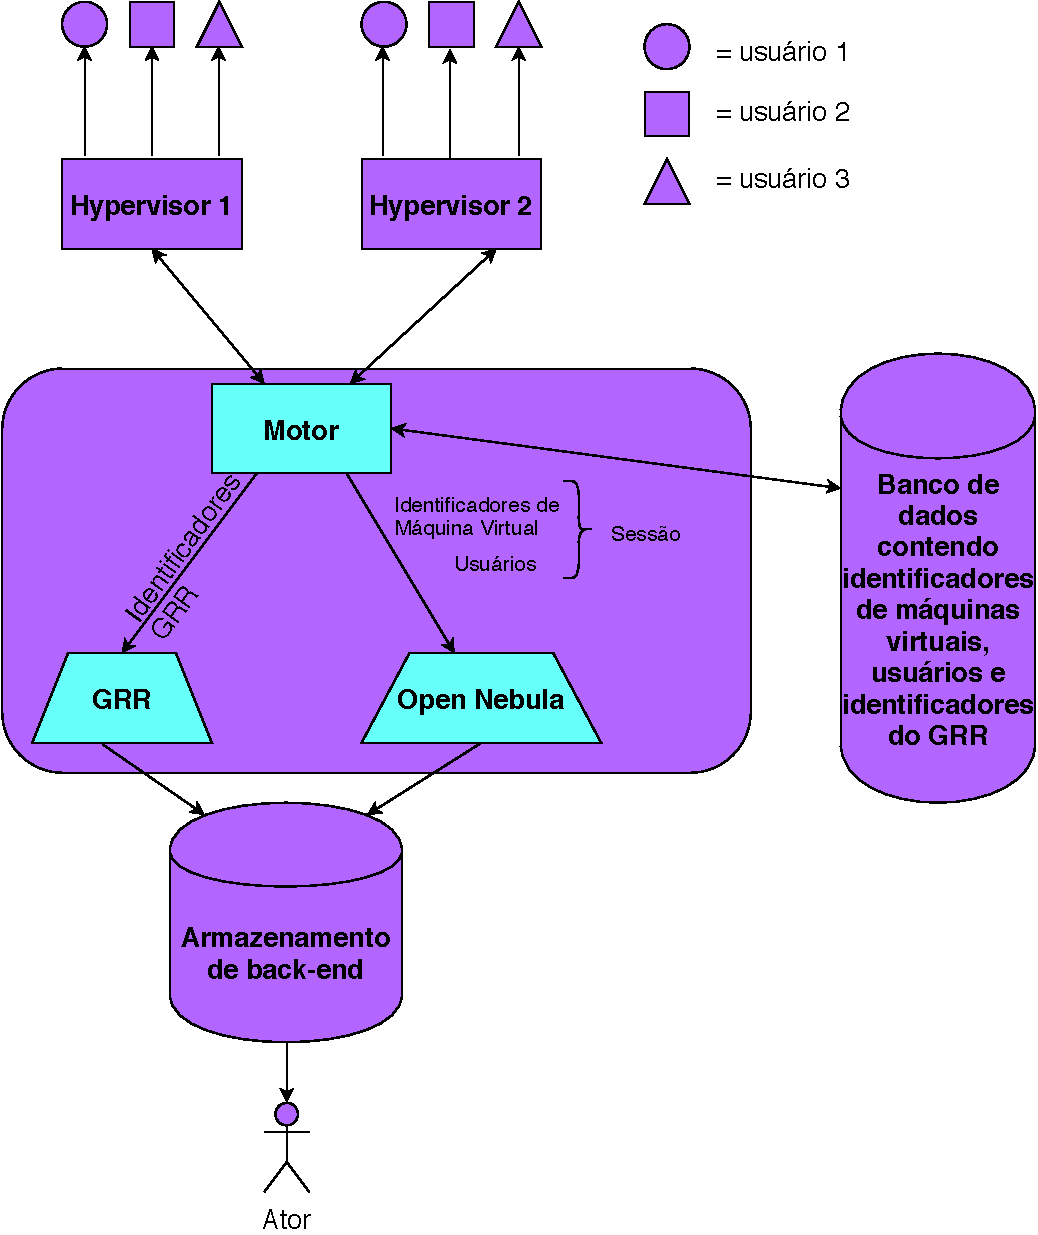
\includegraphics[scale=0.70]{ReichertAutoAcquisitionModel.pdf}
\centering
\label{fig:ReichertAutoAcquisitionModel}
\begin{center}
Adaptado de \cite{ReichertAutoAcquisition:2015} 
\end{center}
\end{figure}


\subsection{Introspecção em máquina virtual}
\label{sec:VMI}

A proposta de \cite{PoiselVMI:2013} é baseada na técnica de Introspecção em Máquina Virtual (\textit{Virtual Machine Introspection} -- VMI) para coleta de memória volátil. 
%
Essa técnica se apoia no fato de que o \textit{hipervisor} mapeia os recursos alocados para máquinas virtuais nos recursos físicos correspondentes da máquina hospedeira.
%
Este mapeamento é usado para permitir que a memória volátil copiada da máquina virtual seja reconstruída em uma máquina física, para análise posterior.
%
A proposta realiza coleta contínua de instantâneos de memória durante o funcionamento do sistema, sem distinção do que aconteceu antes ou depois do fato de interesse, e todos os instantâneos de memória são armazenados para análise.
%
Visando eliminar a chance de inconsistências no instantâneo de memória volátil, a máquina virtual tem sua execução suspensa durante o processo de extração.


Em \cite{PoiselVMI:2013}, no capítulo 3.1, o próprio autor menciona que a necessidade de tradução de endereços de memória da máquina virtual em endereços de memória da máquina física hospedeira dificulta a utilização da técnica em larga escala.
%
Como essa tradução depende de conhecimento do que está sendo executado na máquina virtual, uma solução baseada em VMI não é completamente portável, sendo necessárias adequações para diferentes clientes.
%
Além disso, esta tradução de endereços pode ser computacionalmente custosa.%\marcos{É isso mesmo? Não ficou claro na frase original o que era ``computacionalmente custoso'', então assumi aqui que é ``a tradução''. - Hamilton: sim era mas você tem razão, mudei}.
%

\subsection{Virtuoso}
\label{sec:virtuoso}

Também na vertente de introspecção de máquina virtual, \cite{Dolan-GavittSemanticGap:2011} propõe o \textit{Virtuoso}, um arcabouço de coleta de informações de processos específicos em uma máquina virtual.
%
O arcabouço funciona em três fases.
%
A primeira realiza um estudo em uma máquina virtual de testes, mapeando o conjunto de instruções executado pelo processo do qual se deseja coletar dados de memória. 
%
O estudo é realizado no Ambientes de Treino e o Leitor de Instruções coleta e armazena as instruções geradas pelo processo alvo da análise e os armazena no banco de dados de Instruções Armazenadas.
%
Na segunda fase, o Analisador de Instruções cria um executável a partir do conjunto de instruções coletado na fase anterior. Estas instruções precisam ter suas referências de memória traduzidas para que seja possível executá-las fora do ambiente original, o que ocorre no Tradutor de Instruções.
%
Com o executável, a terceira fase usa um Ambiente Virtual Seguro na máquina hospedeira capaz de acessar os endereços de memória do Ambiente Virtual Não Confiável, tornando possível coletar instantâneos de memória do processo em execução.
%
A Figura \ref{fig:Dolan-GavittSemanticGap} ilustra o funcionamento desse arcabouço. 


A característica deste modelo que mais contribui para a forense digital é a capacidade de coletar instantâneos de memória de um processo específico e reproduzí-lo em um ambiente confiável. Entretanto  sua atuação se dá apenas após o evento que se deseja avaliar forensicamente.
%


\begin{figure}[htb!]
\footnotesize
\caption{Virtuoso}
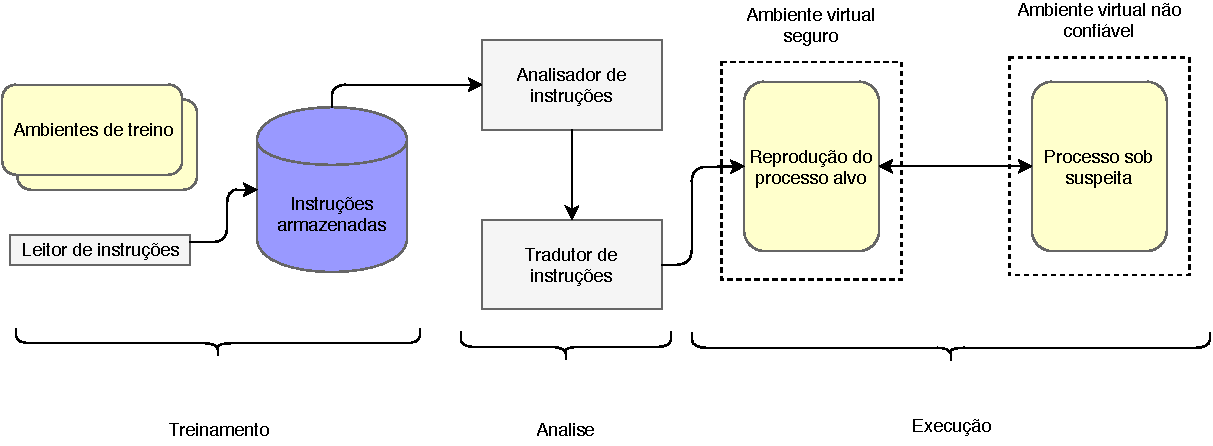
\includegraphics[scale=0.70]{Dolan-GavittSemanticGap.pdf}
\centering
\label{fig:Dolan-GavittSemanticGap}
\begin{center}
Adaptado de \cite{Dolan-GavittSemanticGap:2011} 
\end{center}
\end{figure}


\subsection{Abordagem baseada em logs}
\label{sec:modelologs}

O arcabouço proposto por \cite{SangLogApproach:2013} é um sistema que funciona em parceria com o provedor de nuvem: o provedor último envia informações ao arcabouço, que por sua vez as armazena em um local adequado, de forma centralizada.
%
O conjunto de informações armazenadas é negociado antecipadamente com o provedor de nuvem, indo desde instantâneos de memória volátil até pacotes trafegados nas interfaces de rede da máquina virtual.
%
O arcabouço coleta informações continuamente e usa cálculo de hash das evidências enviadas pelo provedor de nuvem para garantir que elas não foram alteradas durante o transporte.
%
A Figura \ref{fig:SangLogApproach} ilustra o funcionamento da solução, focando em um caso específico de log de rede, de modo similar ao descrito em \cite{SangLogApproach:2013}.


Assim como as propostas anteriores, o arcabouço em questão também não faz distinção do que aconteceu antes ou depois do fato de interesse, mas  coleta constantemente informações da máquina virtual.
%
Outra potencial limitação é que o arcabouço depende da cooperação do provedor de nuvem. 
%
Tal dependência é uma estratégia considerada fraca pela comunidade forense  \cite{ClarkeReviewOfChallenges2015}, pois a prioridade do Provedor de Serviços de Nuvem (\textit{Cloud Service Provider} -- CSP) é a de garantir a disponibilidade do serviço, não de coletar evidências.
%

\begin{figure}[htb!]
\footnotesize
\caption{\textit{A Log Based Approach Model}}
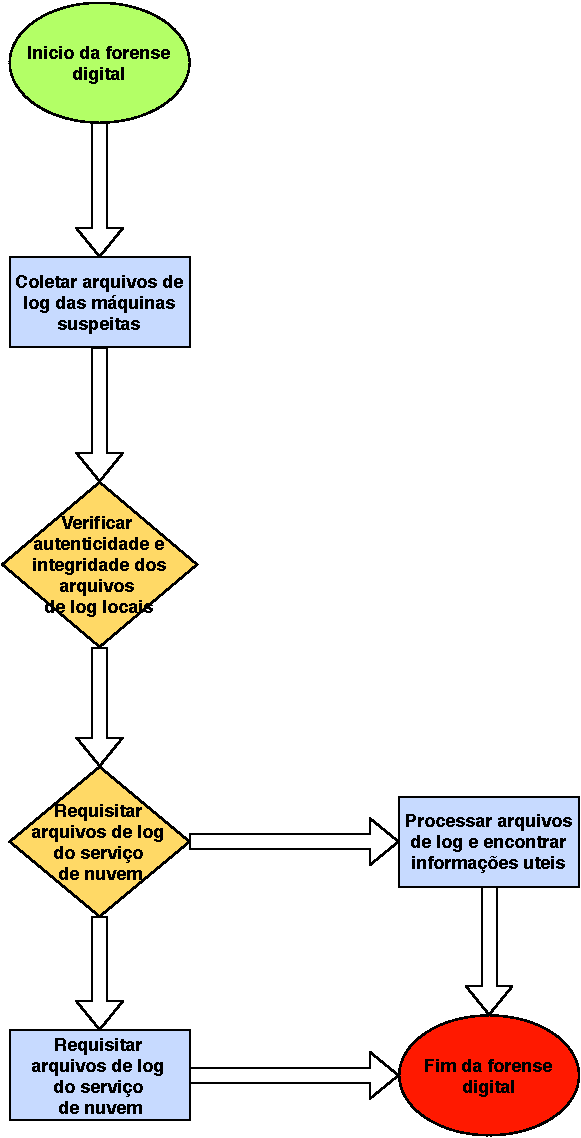
\includegraphics[scale=0.80]{SangLogApproach.pdf}
\centering
\label{fig:SangLogApproach}
\begin{center}
Adaptado de \cite{SangLogApproach:2013} 
\end{center}
\end{figure}


\subsection{Abordagem baseada em backups}
\label{sec:modelobackup}

O trabalho descrito em \cite{DezfouliBackupApproach:2012} é voltado a dispositivos móveis e tem como principal característica a preocupação com as limitações de armazenamento do dispositivo.
%
Por essa razão, o processo de coleta de instantâneos de memória volátil e armazena separadamente as informações de cada processo que está ativo de modo a permitir um gerenciamento adequado do espaço de armazenamento. 
 %
%\marcos{O que seria ``armazenar por processo ativo''? Eu nem sabia que dava para ``armazenar por processo passivo''... - Hamilton: Melhorei}.
%
A solução também se preocupa em descartar informações de processos que foram terminados e removidos da memória, além de buscar o uso consciente do espaço de armazenamento disponível no dispositivo.
%
A Figura \ref{fig:DezfouliBackupApproach} mostra, em alto nível, a forma como o armazenamento de evidências é gerenciado.

Como em diversas outras propostas, processo de coleta de informações de memória volátil em \cite{DezfouliBackupApproach:2012} é executado continuamente, independente de eventos de interesse (e.g., detecção de ameaças). 
%
Um outro fator que conta como desvantagem nesta proposta é o processo não armazenar histórico das coletas anteriores, como é possível ver na Figura \ref{fig:DezfouliBackupApproach}. A coleta anterior é substituída pela nova.
%


\begin{figure}[htb!]
\footnotesize
\caption{\textit{Backup Approach Model}}
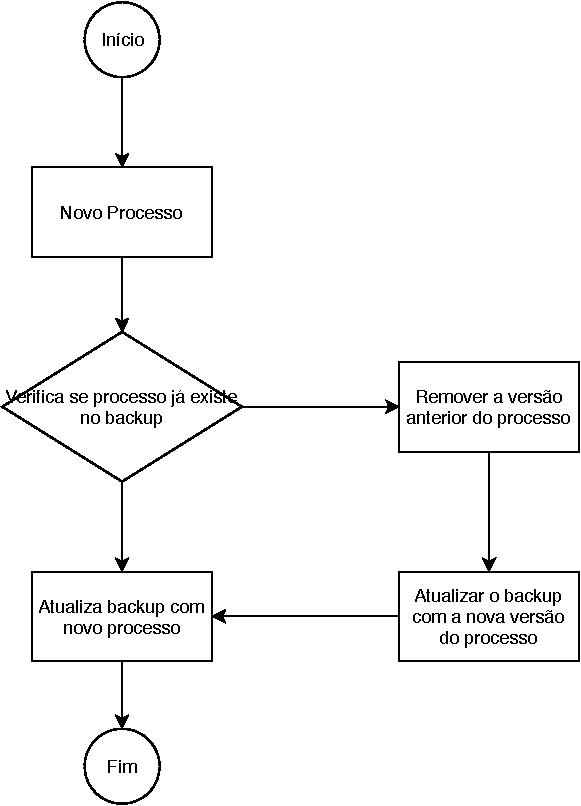
\includegraphics[scale=0.80]{DezfouliBackupApproach.pdf}
\centering
\label{fig:DezfouliBackupApproach}
\begin{center}
Adaptado de \cite{DezfouliBackupApproach:2012} 
\end{center}
\end{figure}


\subsection{Arcabouço forense para OpenStack}
\label{sec:frost}

As Ferramentas Forenses para Arcabouço OpenStack (\textit{FoRensic OpenStack Tools} -- FROST), proposta por \cite{DykstraFROST:2013}, consiste em um conjunto de bibliotecas integradas ao OpenStack, um dos arcabouços de gerenciamento de infraestruturas virtualizadas bastante difundido \cite{StackFramework:2018}.
%
Por meio dessa integração, o FROST expõe um conjunto de APIs que podem ser usadas por aplicações de coleta de evidências forenses.
%
Essas APIs dão acesso a recursos da máquina virtual administrada, tais como disco, \textit{logs} de tráfego de rede e memória volátil.
%
A proposta descreve apenas o arcabouço, deixando a critério do usuário detalhes como periodicidade e tamanho da coleta, bem como a forma de transporte da evidência e onde ela é armazenada.

\begin{figure}[htb!]
\footnotesize
\caption{\textit{FoRensic OpenStack Tools}}
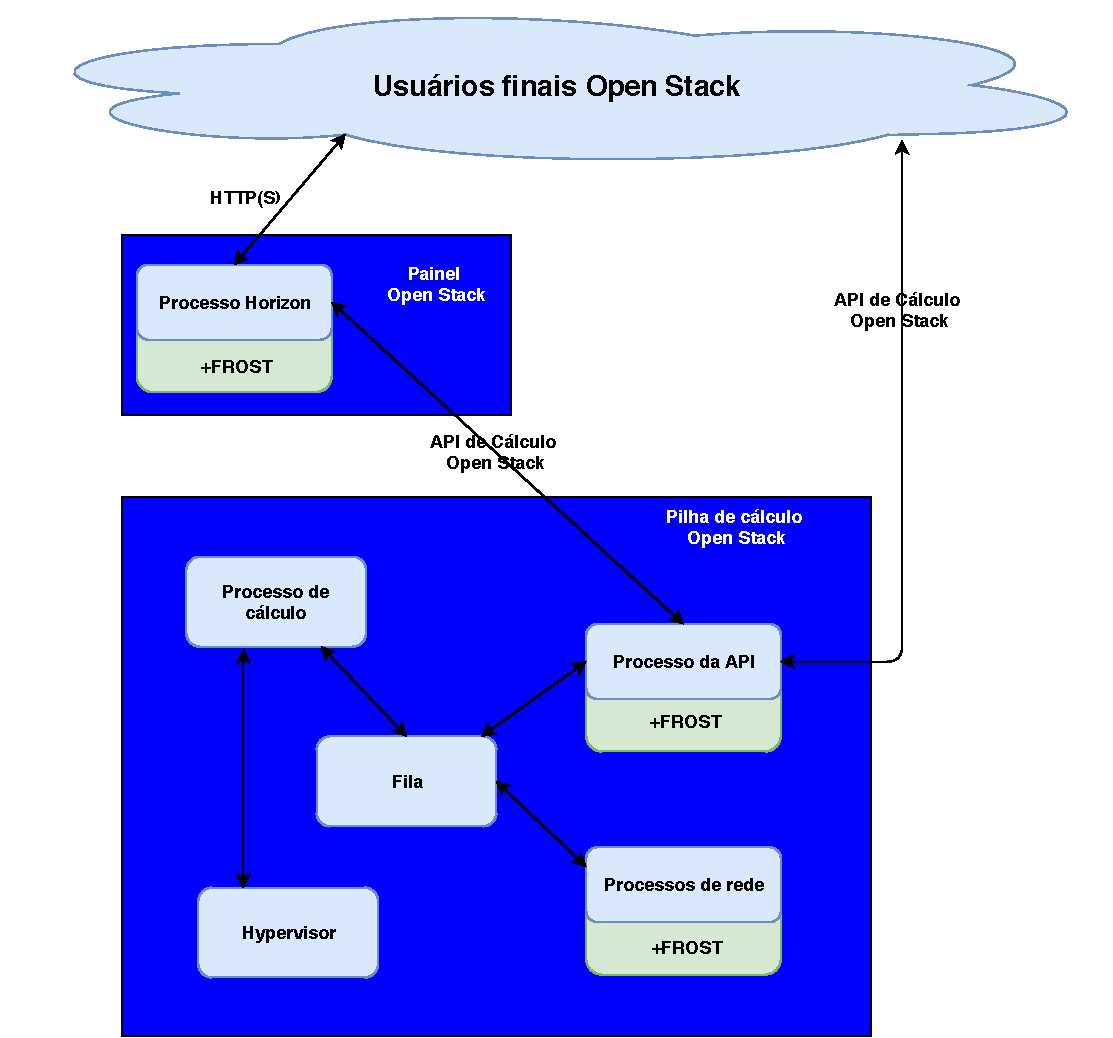
\includegraphics[scale=0.80]{DykstraFROST.pdf}
\centering
\label{fig:DykstraFROST}
\begin{center}
Adaptado de \cite{DykstraFROST:2013} 
\end{center}
\end{figure}
%

A Figura \ref{fig:DykstraFROST} ilustra a integração entre FROST e o arcabouço OpenStack.
%
Nela é possível ver os dois pontos desta integração. O primeiro em sua camada de interface de administração web, através da API de Computação (\textit{Compute API}) onde o usuário pode acionar a coleta de artefatos para análise.
%
A segunda ocorre em seu núcleo, adiciona novas chamadas a API Nova (\textit{Nova API}) do OpenStack para viabilizar a coleta de informações da máquina virtual e também integra com os processos de rede para extrair logs de tráfego da rede.


O autor declara que FROST segue as práticas definidas no Grupo de Pesquisa Cientifica Em Evidência Digital (\textit{Scientific Working Group on Digital Evidence} -- SWGDE) e do Manual de Busca e Apreensão do Departamento de Justiça Norte-Americano \cite{DykstraFROST:2013}.
%
De todas as propostas avaliadas, a FROST é a única que mostra preocupação com adequação a questões legais como cadeia de custódia e integridade da evidência.
%

\subsection{Forense como serviço}
\label{sec:frost}

O trabalho descrito em \cite{GeorgeDF2CE:2012} se concentra em monitoramento de rede, operando em uma arquitetura de Forense Como Serviço (\textit{Forensics as a Service} -- FaaS). 
%
Conforme ilustrado na Figura \ref{fig:GeorgeDF2CE}, a arquitetura da solução consiste em um conjunto de ferramentas com capacidade de descobrir automaticamente as interfaces sob monitoramento, além de coletar evidências de tais máquinas e armazená-las.


O processo de autodescoberta e associação das evidências com usuários de rede é realizado por um motor baseado em ontologias armazenadas em um banco de dados próprio. 
%
As ontologias são utilizadas para determinar a associação entre as evidências coletadas e os usuários ou artefatos que as geraram.
%
O Minerador de dados implementa um algoritmo de descoberta de arquivos de \textit{log} de artefatos de rede definidos como relevantes.
%
O Monitor de rede é responsável por interceptar o tráfego entre as partes consideradas suspeitas e por fim, a Monitoração do Sistema em Tempo Real captura informações específicas do sistema em execução como instantâneos dos processos sob investigação.
%
Entretanto, a proposta se concentra apenas no processo de coleta, enquanto a descrição dos mecanismos de armazenamento e transporte não é detalhada.


\begin{figure}[htb!]
\footnotesize
\caption{\textit{Digital Forensic Framework for Cloud Environment}}
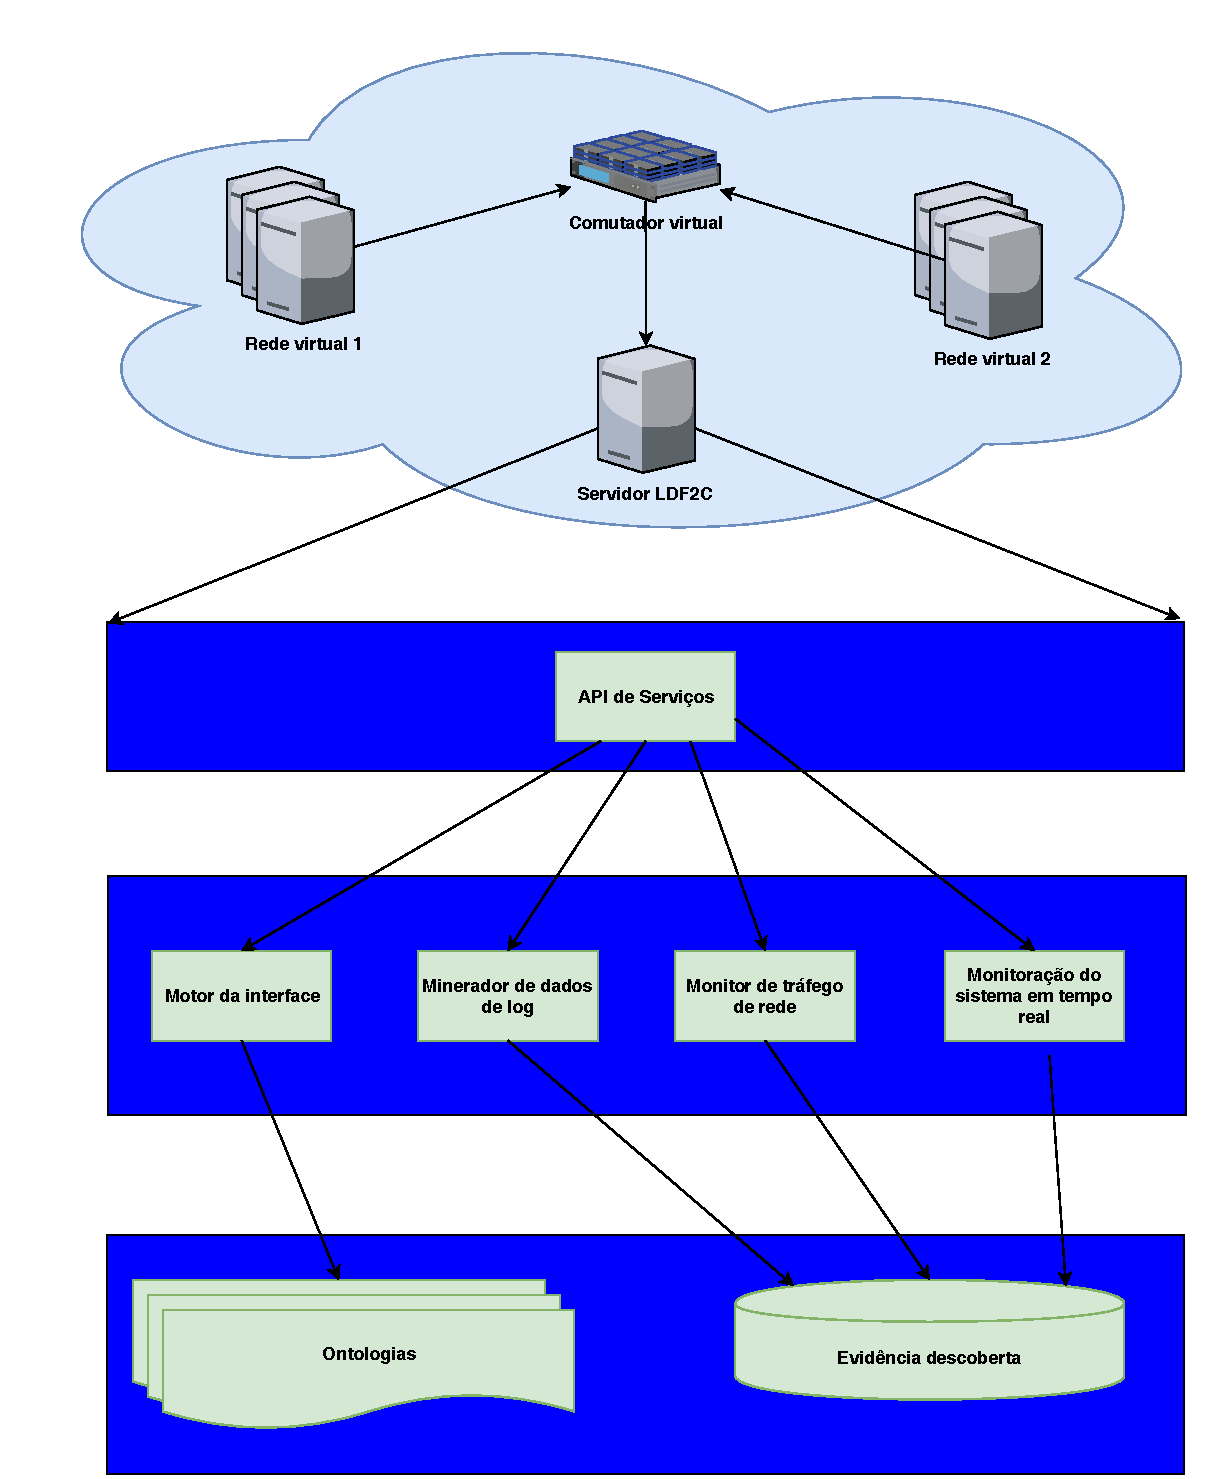
\includegraphics[scale=0.70]{GeorgeDF2CE.pdf}
\centering
\label{fig:GeorgeDF2CE}
\begin{center}
Adaptado de \cite{GeorgeDF2CE:2012} 
\end{center}
\end{figure}


\subsection{Abordagem de indexação de dados coletados para fins forenses}
\label{sec:indexacaoforense}

Na mesma vertente da solução de forense como serviço descrita na Subseção \ref{sec:frost}, \cite{FaaSIndexedSearch:2012} trata o problema de grande volume de dados coletados por meio de um serviço de coleta e indexação de evidências.
%
O serviço espera receber dados da execução do comando unix DD \cite{UnixManPagesDD} nas máquinas alvo, nas quais, apoiado em processos de Extrair, Transformar e Carregar (\textit{Extract, Transform and Load} -- ETL) e MapReduce \cite{MapReduce:2008}, os dados são disponibilizados para consulta pelos investigadores.
%
A coleta ocorre continuamente, em intervalos de tempo configuráveis.


A Figura \ref{fig:FaaSIndexedSearch} mostra a arquitetura da solução. Um Armazenamento Acessado via Rede (\textit{Network Accessed Storage} -- NAS) é usado para armazenar as evidências coletadas.
%
Antes da análise dos dados pelos processos de MapReduce é necessário executar o processo de ETL para adequar a informação a necessidade específica da investigação. Esta fase ocorre nos Nós Filtrando.
%
Em seguida a informação é submetida ao processo de MapReduce e armazenado em um HBase \cite{Hbase2018}.
%
O Nó Mestre tem o papel de orquestrador enviando os comandos de indexação dos dados coletados e recebendo as requisições de busca dos usuários via seu Servidor Web.


Embora interessante, a solução não deixa claro a localização do armazenamento dos dados coletados, nem quem é responsável pela infraestrutura de armazenamento.
%
Também não é discutido como os dados são transportados até o ponto de armazenamento, nem como garantir que esses dados não sejam alteramos no processo.
%


\begin{figure}[htb!]
\footnotesize
\caption{\textit{Digital Forensic as a Service - Indexed Data}}
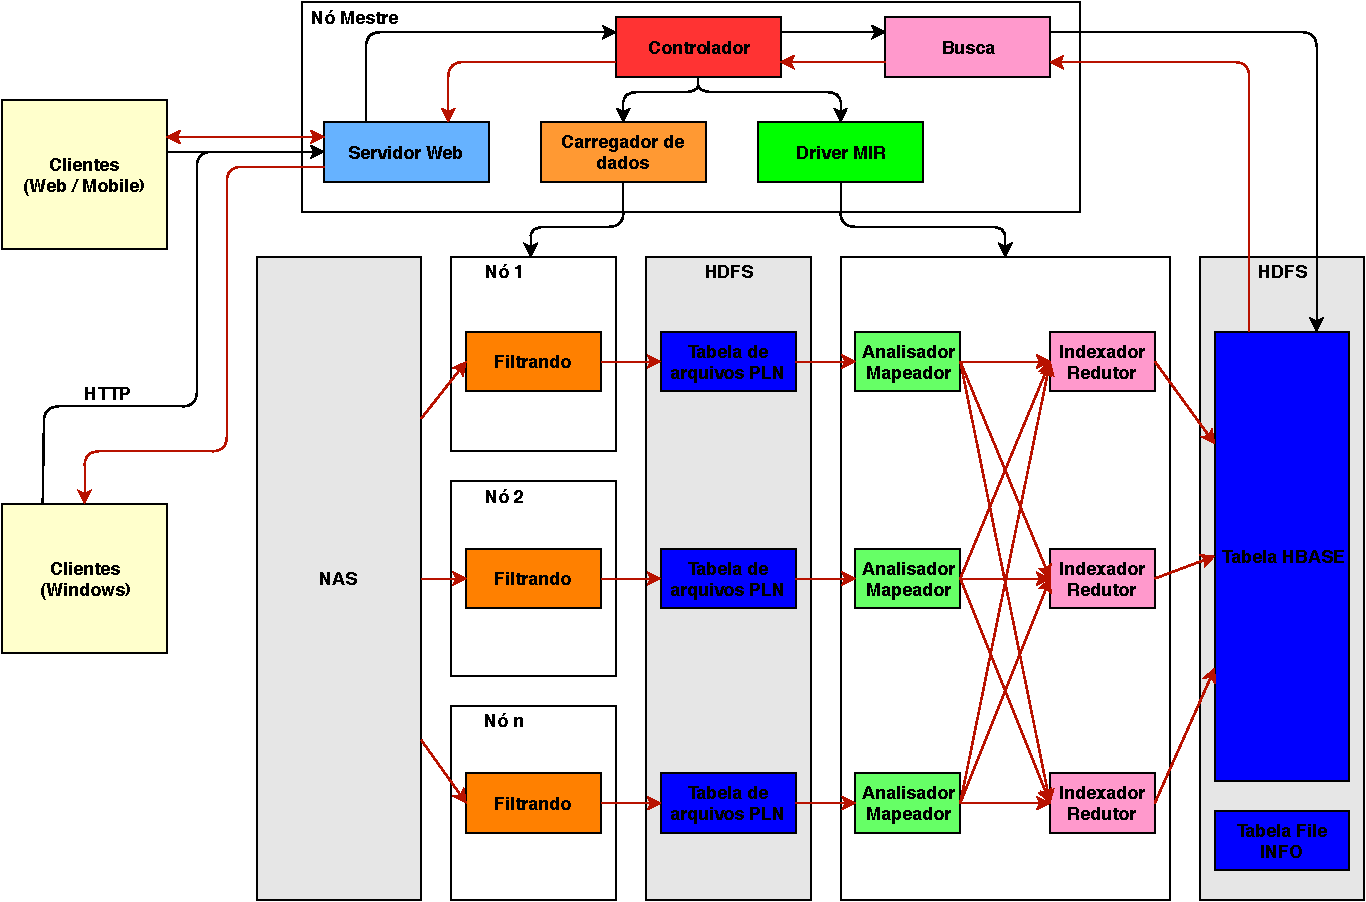
\includegraphics[scale=0.60]{FaaSIndexedSearch.pdf}
\centering
\label{fig:FaaSIndexedSearch}
\begin{center}
Adaptado de \cite{FaaSIndexedSearch:2012} 
\end{center}
\end{figure}


\section{Aspectos relacionados a coleta de evidência}
\label{sec:coletadeevidencia}

Para uma discussão mais estruturada, nas próximas subseções os trabalhos mencionados na Subseção \ref{sec:VMI} são agrupados e avaliados com base nos diferentes aspectos que abordam.

\subsection{Acessar e coletar as informações de memória das máquinas virtuais em nuvem}
\label{sec:coletadeevidencia}

Diversos trabalhos de análise forense na nuvem se concentram na coleta de dados ``após o fato'', ou seja, após a intrusão ser detectada \cite{ReichertAutoAcquisition:2015,PoiselVMI:2013,DykstraFROST:2013,GeorgeDF2CE:2012,SangLogApproach:2013}. 
%
Os processos de coleta descritos nesses trabalhos podem ser iniciados de forma manual ou automaticamente, via integração com um mecanismo de detecção de intrusão. 
%
No caso específico de memória volátil, tal forma de coleta não consegue descrever como era a memória antes da intrusão, pois o processo só é acionado depois da detecção do ataque. 
%
%A capacidade de saber como era a memória antes do fato é descrita por \cite{Case_Memory_Forensics:2014} como necessária para viabilizar a abordagem de coletar o suficiente para realizar a investigação pois permite comparar dois instantâneos de memória e minimizar o volume coletado antes do fato. 
Tal limitação pode trazer prejuízos à investigação, dado que algumas análises dependem exatamente da capacidade de se comparar dois momentos da memória \cite{CaseMemoryForensics:2014}. 
%
Entre os trabalhos estudados, a única proposta encontrada que leva tal necessidade em consideração é \cite{DezfouliBackupApproach:2012}, que propõe que o dado seja armazenado no próprio equipamento sob análise.
%
%Infelizmente, entretanto, essa abordagem não é aplicável ao cenário em nuvem, pois leva a perda de informações importantes caso a máquina virtual seja despejada e seus recursos liberados.
Infelizmente, entretanto, a aplicação de tal abordagem no cenário em nuvem é pouco viável, pois pode levar à perda de informações importantes caso a máquina virtual ou contêiner seja desativada, tendo seus recursos liberados.
%

%Ainda na coleta de informações, os autores \cite{Reichert_Auto_acquisition:2015} e \cite{George_DF2CE:2012} sugerem a abordagem de forense ao vivo onde os dados são constantemente coletados sem distinção do antes ou depois do fato. 
Existem ainda trabalhos voltados à coleta de informações durante a execução do sistema, nos quais os dados são constantemente coletados sem distinção do que aconteceu antes ou depois do fato de interesse.
%
Esse é o caso de trabalhos como \cite{PoiselVMI:2013,DykstraFROST:2013,SangLogApproach:2013,Dolan-GavittSemanticGap:2011}, que adotam a estratégia de isolar e parar a máquina virtual para em seguida realizar o processo de coleta. 
%
%Nas duas estratégias citadas anteriormente, o problema do grande volume de informações coletadas não é abordado pelo autores nem o cenário onde é necessário coletar evidências de uma máquina virtual que já foi despejada do pool e os recursos liberados. 
Embora interessantes, as abordagens descritas nesses trabalhos podem levar a um elevado volume de dados coletados.
%
Além disso, elas não tratam o cenário em que é necessário coletar evidências quando são liberados os recursos virtuais que as contêm.


\subsection{Capacidade de reproduzir o processo e obter os mesmos resultados}
\label{sec:reprodutibilidade}

Se, durante uma análise forense, analistas diferentes obtêm resultados distintos ao executar o mesmo procedimento de coleta, a evidência gerada não tem credibilidade, inviabilizando seu uso em um processo legal. 
%
Por essa razão, a reprodutibilidade do processo de coleta é uma parte importante da geração de evidências para análise forense.
%
Infelizmente, entretanto, nenhuma das propostas encontradas na literatura atualmente permite tal reprodutibilidade em cenários de nuvem, em que máquinas virtuais ou contêineres são desativados e seus recursos físicos liberados.
%
Afinal, todas elas dependem da existência do recurso virtual para a repetição do processo de coleta.

\subsection{Não violar privacidade ou jurisdição das partes não envolvidas na investigação}
\label{sec:legais}

Em um ambiente de nuvem pública, remover o \textit{hardware} para análise posterior pode levar à violação de privacidade de usuários pessoa física e jurídica.
%
A razão é que o multi-inquilinato desse cenário faz com que uma mesma máquina física guarde informações de diversos clientes, alguns dos quais podem não estar envolvidos na investigação em curso.
%
Diversos trabalhos na literatura tratam esse problema adequadamente, por meio de duas estratégias principais: a primeira, adotada em \cite{ReichertAutoAcquisition:2015,GeorgeDF2CE:2012,PoiselVMI:2013,DykstraFROST:2013,FaaSIndexedSearch:2012}, consiste em coletar dados pertinentes à investigação e armazená-los fora da nuvem; a segunda, empregada em \cite{SangLogApproach:2013} e que constitui um caso específico de \cite{GeorgeDF2CE:2012}, depende da cooperação do provedor de serviços de nuvem para conseguir as informações necessárias à investigação. 
%
Depender do provedor de serviços de nuvem é uma estratégia pouco recomendada  \cite{ClarkeReviewOfChallenges2015}, entretanto, pois (1) o volume de dados de usuários pode forçar os provedores a limitar o tamanho dos \textit{logs} armazenados, e (2) caso ocorra uma indisponibilidade causada por um ataque, o objetivo do provedor será o de restabelecer o serviço, não necessariamente o de preservar evidências. 


\subsection{Garantir a cadeia de custódia da evidência}
\label{sec:cadeiadecustodia}

Dentre os trabalhos analisados, apenas \cite{SangLogApproach:2013} aborda a questão da garantia da cadeia de custódia. 
%
Especificamente, o trabalho emprega \textit{hashes} para verificar a integridade da evidência, permitindo a detecção de alterações.
%
Uma limitação desse trabalho, entretanto, é que ele não deixa explícitos os mecanismos que poderiam ser utilizados para impedir acesso não autorizado (e, assim, potencial alteração) aos próprios \textit{hashes}. 
%
As propostas dos outros autores concentram-se apenas no aspecto técnico da coleta, sem discutir detalhadamente garantia de custódia.
%
Em geral, os trabalhos apenas mencionam que as evidências devem ser coletadas de forma forensicamente aceitável.

\section{Resumo}
\label{sec:resumo}

A Tabela \ref{tab:related-work} mostra um comparativo das soluções estudadas, considerando os aspectos discutidos nesta seção, posicionando as contribuições da proposta apresentada neste trabalho.

\begin{table}[htb!]
\footnotesize
\renewcommand{\arraystretch}{1.4}
\renewcommand{\tabcolsep}{0.5mm}
\centering
\caption{Comparativo de soluções de coleta de informações de memória de máquinas em nuvem para análise forense}
\label{tab:related-work}
\begin{tabular}{p{5.3cm}|L|L|L|L|L|L|L|L|L|}
\textbf{}						& \rot{\fancyname~(esta proposta)} 			& \rot{\cite{GeorgeDF2CE:2012}} 
							& \rot{\cite{PoiselVMI:2013}} 				& \rot{\cite{DykstraFROST:2013}}
							& \rot{\cite{FaaSIndexedSearch:2012}} 			& \rot{\cite{ReichertAutoAcquisition:2015}}	
							& \rot{\cite{SangLogApproach:2013}} 			& \rot{\cite{Dolan-GavittSemanticGap:2011}} 
							& \rot{\cite{DezfouliBackupApproach:2012}} 				
\\ \hline
\textbf{Coleta evidência continuamente.}		& \cfig	& \xfig & \xfig & \xfig & \cfig & \xfig & \cfig & \xfig & \cfig  \\
\textbf{O processo é reprodutível.}		& \cfig	& \xfig & \xfig & \xfig & \xfig & \xfig & \xfig & \xfig & \xfig  \\
\textbf{Garante cadeia de custódia.}			& \cfig	& \xfig & \xfig & \xfig & \xfig & \cfig & \cfig & \xfig & \xfig  \\
\textbf{Preserva privacidade e jurisdição.} 		& \cfig	& \cfig	& \cfig	& \cfig	& \cfig	& \cfig	& \cfig	& \cfig	& \cfig	 \\
\end{tabular}
\end{table}

% ----------------------------------------------------------
% Proposta
% ----------------------------------------------------------
\chapter{Proposta de projeto: \fancyname}
\label{chp:proposta}

A presente proposta tem como objetivo principal coletar memória de recursos computacionais virtuais em arquitetura volátil de modo a conseguir: 
(1) identificar a fonte da evidência, mesmo se o recurso virtual não existir mais e assim conseguir reproduzir o processo de coleta; 
(2) descrever o sistema antes e depois do incidente mantendo sob controle a quantidade de dados coletados;
(3) transportar e armazenar a memória coletada de uma forma que garanta a cadeia de custódia; e
(4) não violar a jurisdição e a privacidade de outros usuários que porventura tenham recursos alocados no mesmo servidor físico.
%
A solução aqui apresentada, denominada \fancyname, é descrita em detalhes nas próximas subseções.

\section{Identificação da origem}
\label{sec:proposal-desc-origin}

Em sistemas computacionais executados sobre uma infraestrutura física (i.e., não virtualizada), pode-se fazer uma associação direta entre um recurso qualquer e sua origem correspondente, seja este recurso uma informação da memória, imagem de disco ou pacotes trafegando na rede.
%
Já em sistemas construídos sobre uma infraestrutura virtual, em especial quando ela é auto-escalável, os recursos computacionais são altamente voláteis e, portanto, podem ser desalocados a qualquer momento.
%
Este fato torna difícil a associação de uma informação gerada por esta infraestrutura com sua origem.


Para conseguir correlacionar uma evidência a sua origem volátil, é necessário utilizar outro elemento em que persista a relação fonte-evidência.
%
O presente trabalho propõe que isto seja feito por meio de cálculo de \textit{hash} do recurso em nuvem que produziu a evidência. %removendo contêiner para deixar mais genérico
%
%Embora um contêiner seja um \textit{software} e, portanto, também volátil, cada imagem compilada e sua execução na forma de contêiner são normalmente atrelados a um \textit{hash} que identifica univocamente essa relação. %removendo para deixar mais genérico
%
O \textit{hash} de um recurso em nuvem permite identificar univocamente a fonte de uma evidência. Em arquiteturas que utilizam contêiner por exemplo, é possível identificar se a evidência veio do contêiner do motor de páginas dinâmicas (e.g., Apache%\cite{Tomcat}
), do contêiner da lógica de negócios (e.g., \textit{golang}%\cite{Google}
) ou do contêiner do banco de dados (e.g., \textit{Cassandra}%\cite{Cassandra}
). %removendo contêiner e deixando mais genérico

\section{Descrever o sistema antes e depois do incidente}
\label{sec:proposal-desc-incident}

%\marcosT{O parágrafo estava muito grande, então quebrei aqui. O problema é que falta uma frase para ligar a frase a seguir ao contexto da discussão... Coloque uma frase aqui, deixando claro qual requisito você quer satisfazer com essa ideia de ``interromper temporariamente a execução do contêiner''. Aplique isso para TUDO que for proposta: o leitor tem que saber de antemão pra que você está fazendo alguma coisa, ou vai ficar se perguntando ``Espera, mas pra que fazer isso?!'' - Hamilton: Feito}
A cópia de memória não é uma atividade atômica, pois ela é executada em conjunto com outros processos. 
%
Portanto, caso um desses processos seja um código malicioso apagando traços de sua existência da memória do recurso, informações possivelmente importantes para a investigação podem acabar sendo perdidas. 
%
Com o objetivo de deixar o processo de cópia da memória mais atômico, a fim de evitar inconsistências na informação coletada \cite{CaseMemoryForensics:2014}, \fancyname propõe que a execução do recurso em nuvem seja temporariamente suspenso para que seja realizada a cópia de sua memória. 
%
Essa técnica, que é semelhante àquela adotada em \cite{RafiqueStaticLiveDigitalForensics:2013} para VMs, produz um instantâneo da memória volátil do recurso; isso permite sua análise em um estado de repouso, ou seja, sem a necessidade de ter o recurso em execução.
%
Ao realizar a coleta em intervalos de tempo adequados, é possível construir um histórico do estado da memória durante a execução no recurso.
%
%\marcosT{A ligação entre as frases anterior e a seguir está bem ruim... você parece estar mudando completamente de assunto... Acredito que faltou uma frase dizendo que ``''salvar toda a memória'' pode se tornar um problema, reforçar isso com as duas frases que já estão a seguir, e depois dizer que você vai resolver.}

\begin{figure}[htb!]
\footnotesize
\caption{Janela deslizante de coleta de evidência}
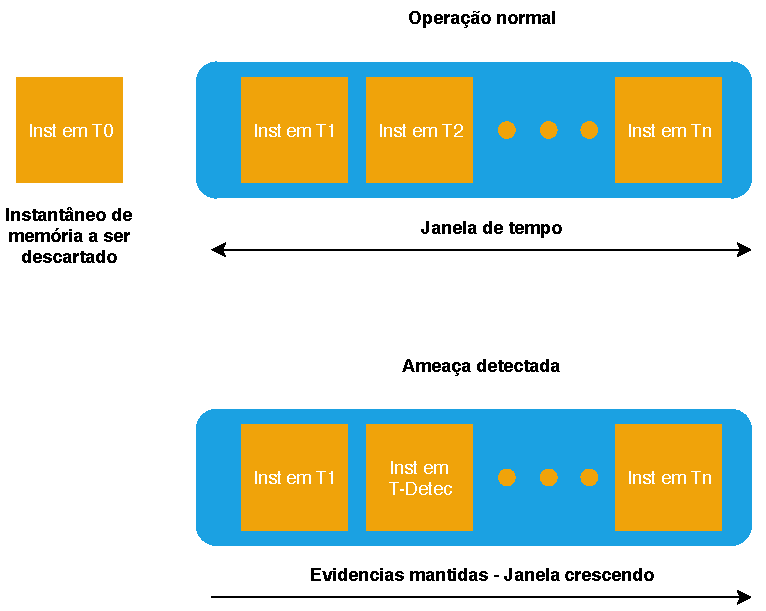
\includegraphics[scale=1.00]{janela.pdf}
\centering
\label{fig:janela}
\begin{center}
Fonte: Próprio autor 
\end{center}
\end{figure}

A maioria das técnicas forenses mais usadas atualmente são voltadas à obtenção da informação em sua totalidade.
%
Isso comumente é feito via cópia bit a bit ou por meio da obtenção do \textit{hardware} físico \cite{SimouCloudChlng:2014} \cite{BemPastPresentFuture:2008}. 
%
Embora tais técnicas possam parecer interessantes à primeira vista, estas muitas vezes acabam sendo responsáveis por um problema: o crescente volume de informações que os investigadores precisam analisar \cite{QuickIncreaseVolumeImpact:2014}.
%
Para mitigar essa dificuldade, em \fancyname são adotadas duas estratégias: a primeira é a definição de um volume de dados que possa ser considerado \textit{suficiente} para a realização de uma investigação; a segunda é a definição de uma \textit{idade máxima} para a evidência enquanto o sistema trabalha em condições normais, isto é, quando não está sob ataque.
%
Para detectar e analisar intrusões na memória de processos, é necessário ter uma cópia da memória antes e depois da intrusão \cite{CaseMemoryForensics:2014}. 
%
Assim, a solução proposta implementa uma janela de instantâneos de memória cobrindo um intervalo de tempo pré-definido, como ilustrado na Figura \ref{fig:janela}. 
%
Em condições normais de operação, as evidências são coletadas com certa periodicidade e coletas que atingem uma determinada idade são descartadas.
%
Em contraste, após a detecção de um evento de ataque (e.g., por um sistema de detecção de intrusões), \fancyname deixa de descartar as coletas mais antigas do \textit{log} de monitoramento.
%
Como resultado, é possível conhecer o sistema antes e depois do ataque e, assim, avaliar sua evolução.
%
%\marcosR{Não sei por que você está utilizando $\backslash\backslash$ no final das suas frases, mas pare de fazer isso... deixe o LaTeX se virar com a formatação. No final, quando você tiver tudo escrito, aí pode fazer algum sentido se preocupar com formatação, mas não antes disso... - Hamilton: é pra formatação mesmo :-) OK vou deixar o latex se virar}
%

\section{Garantindo integridade, confidencialidade e protegendo privacidade e jurisdição}
\label{sec:proposal-desc-chain-of-custody}

%\marcosT{Essa frase não faz sentido: não se ``assina'' nada com um ``hash''. Você pode ``calcular o hash'' ou ``assinar um dado'' (e.g., um dado juntamente com o hash de alguma coisa). Revise essa frase... - Hamilton: Feito}
Finalmente, para persistir a relação evidência-origem e garantir a sua integridade, \fancyname calcula o \textit{hash} $H$ do par \{evidência, identificador da imagem do contêiner\} e armazena a tripla \{$H$, identificador do recurso, evidência\}.
%
Adicionalmente, a presente proposta evita eventuais problemas com o armazenamento desses dados em países com jurisdições diferentes daquelas que devem ser aplicadas na investigação em questão.
%
Especificamente, as evidências coletadas são armazenadas em um local físico fora da nuvem, após serem transportadas por meio de um canal seguro (e.g., via TLS (\textit{Transport Layer Security} -- Camada de Transporte Seguro) \cite{DierksT2008}).
%
%Evitando assim problemas de relacionados a falta de acordos de cooperação no combate a crimes digitais entre regiões onde ocorreu o crime e onde a evidência está armazenada.
Dando ao processo de investigação maior celeridade uma vez que a coleta das evidências já terá ocorrido de forma forensicamente aceitável.
%

\section{Implementação}
\label{sec:proposta-impl}

%\marcosT{CLAREZA: quais ataques? Onde estão esses objetivos (diga a seção!!!)? Perceba que não tem qualquer seção com esse nome: você espera realmente que o leitor procure no seu texto onde eles estão...? - Hamilton: Feito}

\begin{figure}[htb!]
\footnotesize
\caption{Arquitetura geral da solução Dizang}
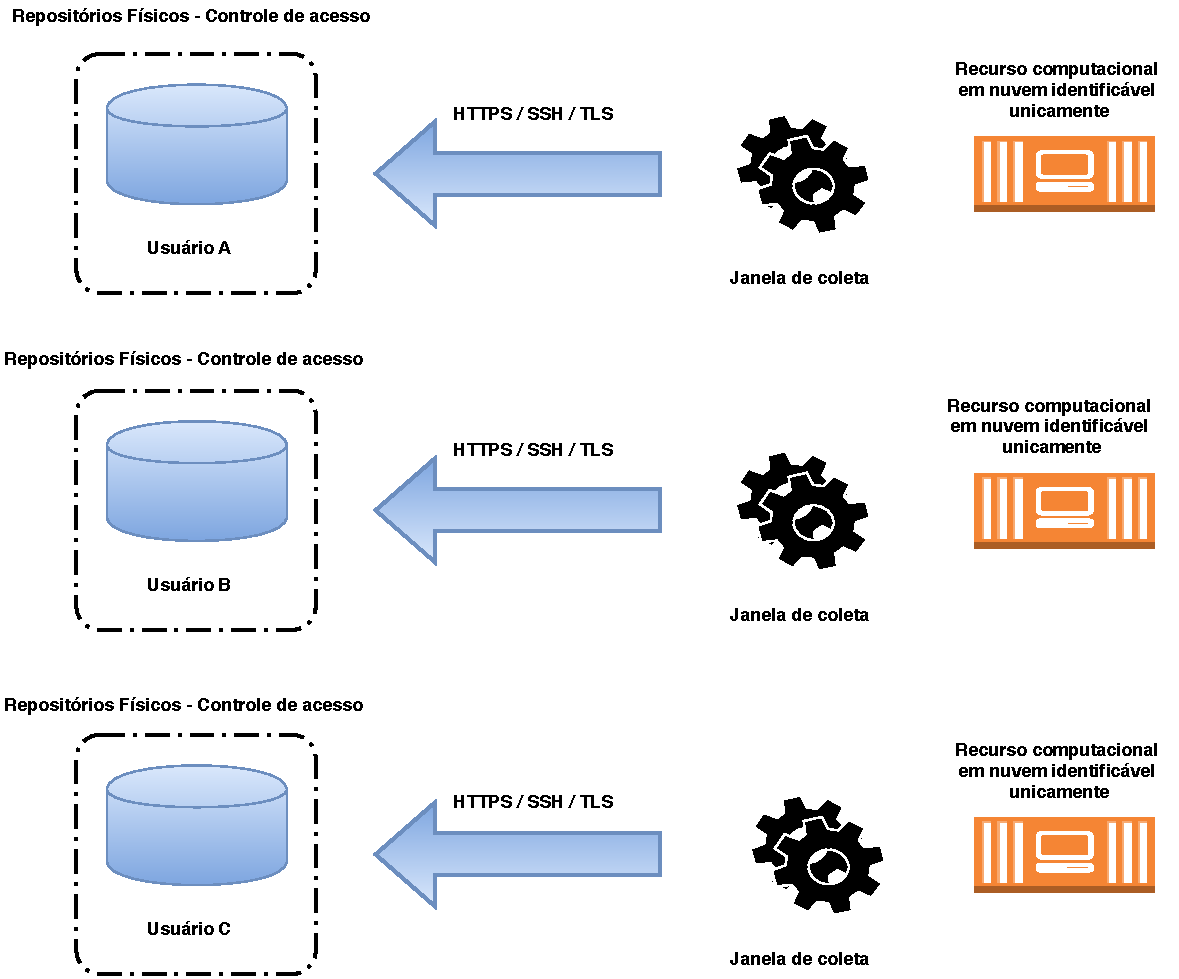
\includegraphics[scale=0.70]{Solucao.pdf}
\centering
\label{fig:Solucao}
\begin{center}
Fonte: Próprio autor 
\end{center}
\end{figure}

%
Os mecanismos propostos foram implementados em uma plataforma de testes visando avaliar a eficácia de \fancyname em coletar as informações de memória dos contêineres de forma reprodutível, sem violar jurisdições ou a privacidade de usuários e a capacidade de detectar injeção de código usando as evidências coletadas.
%
A solução, ilustrada na Figura \ref{fig:Solucao}, consistiu na utilização do serviço EC2 para criação de uma instancia t2.micro Ubuntu Server 14.04 LTS de 64 bits (x86) com armazenamento em SSD na zona Ohio da AWS. 
%na criação de 1 VM usando o Oracle Virtual Box 5.0%\cite{VirtualBox} em um notebook Intel i5 de 2.30Mhz e 4Gb de RAM com sistema operacional de 64 bits.
%
Nesta instância AWS foi manualmente instalado o Docker Engine 1.10 e a API Docker 1.21, com os quais foram criados 3 contêineres executando o Nginx 1.0 em diferentes portas. 
%
Não foram utilizados serviços de contêiner do provedor AWS como EKS ou ECS nos experimentos.
%
Foi desenvolvida uma aplicação Java cujo fluxo é ilustrado na Figura \ref{fig:fluxo-dizang} que, executada no sistema operacional hospedeiro, descobre o identificador de processo associado a cada contêiner, copia o conteúdo do \textit{descritor de alocação de memória não uniforme} (\textbf{/proc/pid/numa\_maps}), o qual contém a alocação das páginas de memória, os nós que estão associados a essas páginas, o que está alocado e suas respectivas políticas de acesso \cite{UnixManPagesNumaMaps}.
%
A cópia e gravação do arquivo é tal que, a cada intervalo de tempo $t$, a aplicação (1) pausa o contêiner em questão, (2) copia a diretório \textbf{numa\_maps}, (3)  concatena os dados obtidos com o identificador da imagem e do contêiner, (4) calcula o $H$ do conjunto e (5) salva o resultado em um arquivo cujo nome é o identificador da imagem e do contêiner e a extensão é \textbf{.mem}. 
%
A pausa do funcionamento do contêiner foi materializado através da chamada a API do Docker, \texttt{http://<docker-url>:<docker-port>/containers/<id-conteiner>/pause} que suspende o funcionamento do contêiner.
%
O transporte seguro da evidência para um armazenamento físico fora da AWS foi implementado usando no serviço EC2, uma instância t2.micro Ubuntu Server 14.04 LTS de 64 bits (x86) com armazenamento em SSD na zona Ohio da AWS no qual foi instalado um servidor \textit{OpenVPN}.
%
Como uma forma básica de controle de acesso, a instância EC2 que contém as evidências foi configurada para aceitar conexões apenas de máquinas nesta VPN.
%
A instância EC2 e a instância da qual foram coletadas as evidências estavam na mesma VPC padrão da AWS
%
Uma máquina física fora da AWS, usou o cliente do \textit{OpenVPN} para estabelecer uma conexão VPN com a instância que contém as evidências e as transportou para o disco da máquina física.
%
A conexão entre a máquina física fora da nuvem e a instância de EC2 na nuvem foi feita utilizando um provedor de banda larga de uso doméstico de 50Gb (Live Tim).
%
Após a conclusão do processo de transporte, a máquina física verifica se existem arquivos \textbf{.mem} em disco mais antigos que um certo intervalo de tempo $t$, descartando-os.
%

\begin{figure}[htb!]
\footnotesize
\caption{Fluxo de execução de Dizang para 1 hospedeiro de contêiner}
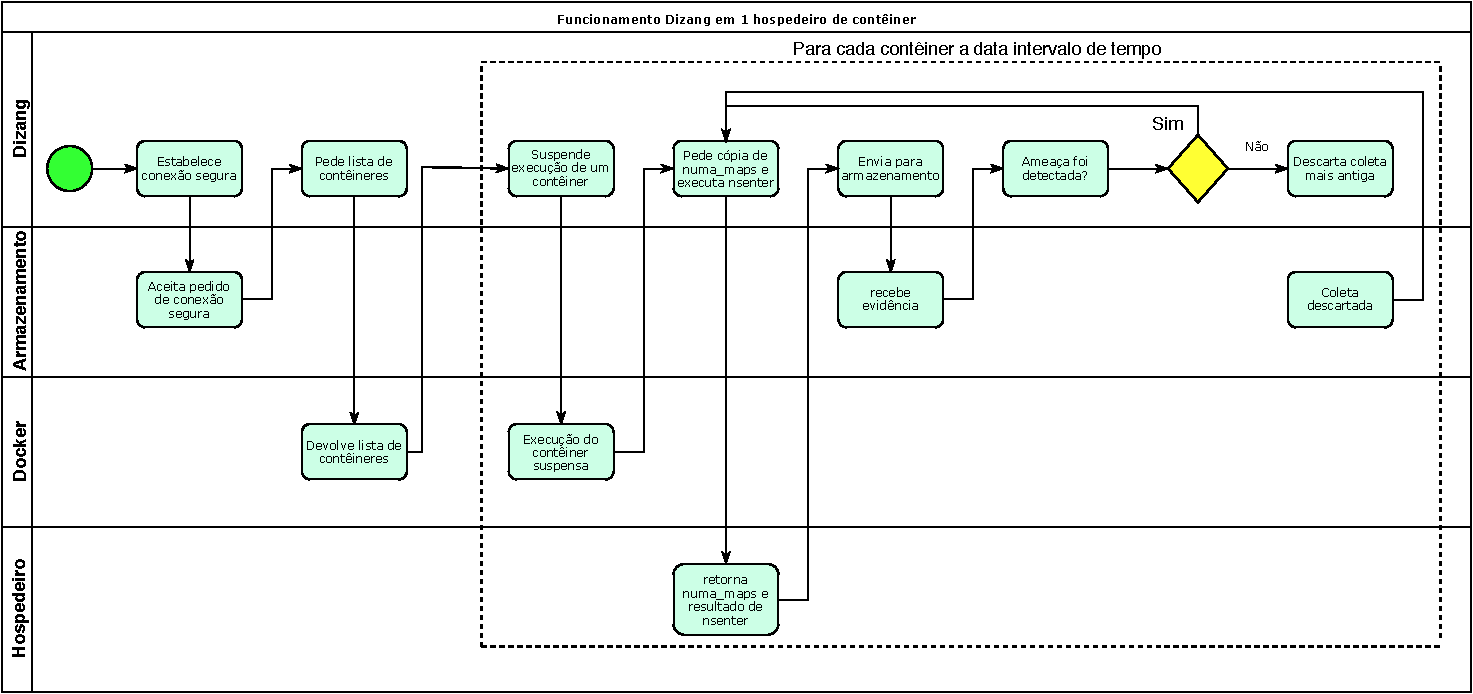
\includegraphics[scale=0.80, angle=270]{Fluxo-Dizang.pdf}
\centering
\label{fig:fluxo-dizang}
\begin{center}
Fonte: Próprio autor 
\end{center}
\end{figure}


\section{Resultados experimentais}
\label{sec:proposta-exp}

Para avaliar a efetividade de \fancyname na coleta de evidências e identificação de injeção de código, dois experimentos foram realizados usando o ambiente implementado (descrito na Seção \ref{sec:proposta-impl}).
%


\subsection{Análise do desempenho}
\label{sec:proposta-exp-desempenho}

No primeiro experimento, o sistema foi configurado para realizar coletas de memória em intervalos de 1 minuto, salvá-las em armazenamento externo à nuvem e apagar amostras coletadas há mais de 5 minutos. 
%
O sistema foi então executado por 30 minutos, tempo durante o qual foram coletadas como métricas (1) o uso de espaço em disco utilizado pelos instantâneos de memória salvos, (2) o tempo de pausa no contêiner necessário para a cópia delas e (3) o tempo de transporte das evidências para o armazenamento externo a nuvem.


A evolução do espaço em disco ocupado pelos instantâneos de memória, acompanhado através da execução do comando \texttt{du -sh *.mem} do \textit{Unix} no disco de armazenamento externo, é mostrada no gráfico da Figura \ref{fig:evolucao-coleta}.
%
Neste experimento os instantâneos de memória tem 244kb de tamanho. 
%
O gráfico mostra que o aumento do uso do espaço de armazenamento é linear e o crescimento se interrompe quando é atingido o limite de tempo configurado para a janela, pois as coletas com tempo de vida maior que tal limite são apagadas do armazenamento final. 
%
Assim, a solução mantém sob controle o espaço em armazenamento ocupado pelas amostras coletadas.
%
Ao mesmo tempo, instantâneos de memória salvos pela solução depois que os contêineres são removidos continuam no armazenamento da máquina, podendo ser associados a sua origem (i.e., contêiner e imagem), conforme esperado para uma análise forense.
%
Essa capacidade se mantém após a detecção de uma ameaça, pois nesse caso coletas mais antigas deixam de ser apagadas.
%
Logo, é possível descrever o estado do sistema antes e depois do incidente \cite{CaseMemoryForensics:2014}, permitindo-se, por exemplo, que ataques de injeção de código em memória sejam analisados.
%

Este experimento usou 3 contêiners para demonstrar que a solução mantém sob controle o espaço em armazenamento ocupado pelas coletas. 
%
Segundo \cite{StubbsConteinersNumberMicroServices:2015} aplicações web modernas são compostas por diversos microserviços implementados em contêiners.
%
Neste cenário, entende-se que o espaço do armazenamento consumido ainda estaria sob controle porém em um patamar mais elevado uma vez que a quantidade de contêiners seria maior.
%


%\marcos{EVITE REDUNDÂNCIA ENTRE GRÁFICO E TABELA. Faz sentido apenas se um deles for trazer informações adicionais (e, nesses casos, em geral o gráfico/tabela acaba tendo algum highlight, para deixar a utilidade dessa redundância)
%\begin{table}[htb!]
%\centering
%\caption{Evolução do uso do espaço em disco}
%\label{tab:results-size}
%\begin{tabular}{c|c}
%\hline
%Tamanho total ocupado (KBytes) & Tempo (segundos) \\ \hline
%240                            & 1                \\ \hline
%480                            & 2                \\ \hline
%720                            & 3                \\ \hline
%960                            & 4                \\ \hline
%1200                           & 5                \\ \hline
%1200                           & 6                \\ \hline
%1200                           & 7                \\ \hline
%1200                           & 8                \\ \hline
%1200                           & 9                \\ \hline
%1200                           & 10                \\ \hline
%1200                           & 11                \\ \hline
%1200                           & 12                \\ \hline
%1200                           & 13                \\ \hline
%1200                           & 14                \\ \hline
%1200                           & 15                \\ \hline
%1200                           & 16                \\ \hline
%1200                           & 17                \\ \hline
%1200                           & 18                \\ \hline
%1200                           & 19                \\ \hline
%1200                           & 20                \\ \hline
%1200                           & 21                \\ \hline
%1200                           & 22                \\ \hline
%1200                           & 23                \\ \hline
%1200                           & 24                \\ \hline
%1200                           & 25                \\ \hline
%1200                           & 26                \\ \hline
%1200                           & 27                \\ \hline
%1200                           & 28                \\ \hline
%1200                           & 29                \\ \hline
%1200                           & 30                \\ \hline
%\end{tabular}
%\end{table}

\begin{figure}[htb!]
\footnotesize
\caption{Evolução do uso do espaço em armazenamento com o Dizang}
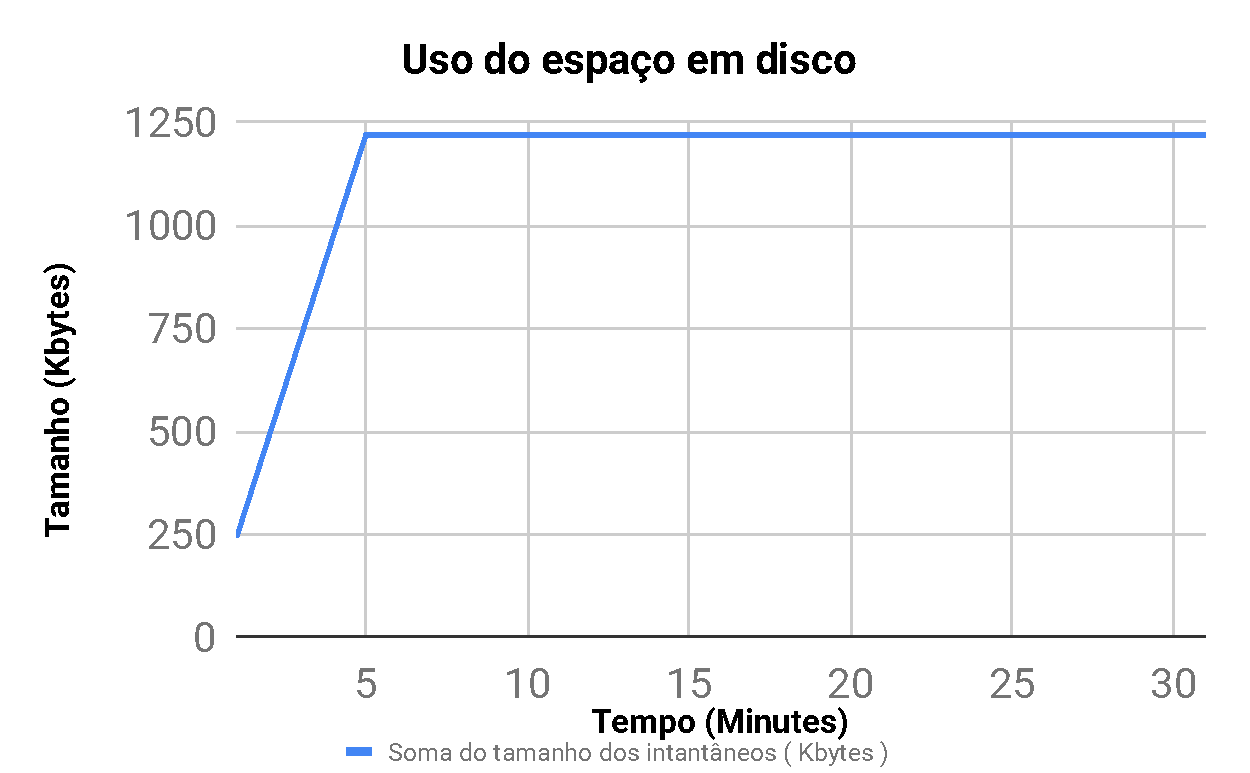
\includegraphics[scale=0.60]{evolucao-coleta.pdf}
\centering
\label{fig:evolucao-coleta}
\begin{center}
Fonte: Próprio autor 
\end{center}
\end{figure}


\begin{comment}
A Figura \ref{fig:memoria_salva}, por sua vez, mostra uma listagem de alguns dos instantâneos de memória salvos pela solução depois que os contêineres são removidos. 
%
Nela pode-se ver que as coletas continuaram no disco da máquina mesmo após a remoção dos contêineres. 
%
Usando o identificador do contêiner e da imagem, consegue-se associar a evidência a sua origem (i.e., a imagem e o contêiner), conforme esperado para uma análise forense.
%
Essa capacidade se mantém após a detecção de uma ameaça, pois nesse caso coletas mais antigas deixam de ser apagadas.
%
Assim, é possível descrever o estado do sistema antes e depois do incidente \cite{Case_Memory_Forensics:2014}, permitindo-se, por exemplo, que ataques de injeção de código em memória sejam analisados.


\begin{figure*}[htb!]
\footnotesize
\caption{Exemplo de lista de instantâneos de memória.}
\fbox{
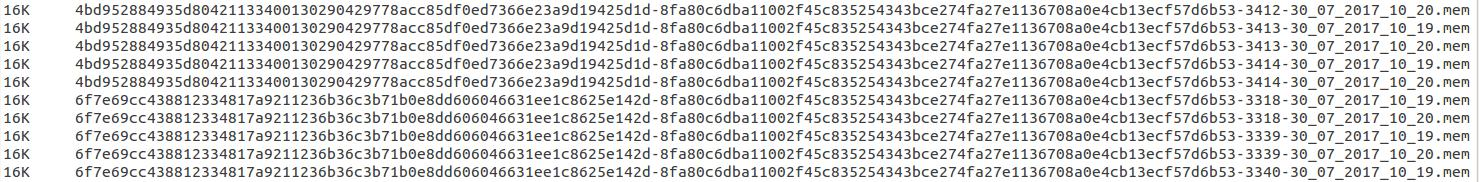
\includegraphics[scale=0.30]{memoria_salva.jpg}
}
\centering
\label{fig:memoria_salva}
\end{figure*}

\end{comment}

%No evento da detecção de uma ameaça a presente proposta deixa de apagar as coletas mais antigas. 
%
%Desta forma é capaz de descrever a história das alterações da memória do contêiner e com isso viabilizar a análise forense em busca das 4 vulnerabilidades de injeção de código em memória citadas no início do artigo. \marcos{Link bem fraco com introdução... pra que explicar em *detalhes* as vulnerabilidades na Introdução se você vai fazer uma explicação *superficial* de como elas são abordadas... Coloquei en passant para não dar a impressão de que você quis chamar a atenção para aquelas vulnerabilidades (sim, eu tinha pedido para você fazer esse link, mas um link tão fraco joga CONTRA você, não a favor...)}
%
%A viabilidade se dá pois consegue descrever o estado do sistema antes e depois do incidente \cite{Case_Memory_Forensics:2014}.
%

Uma potencial limitação da solução proposta é que a pausa de um contêiner para coleta de dados poder, em princípio, causar perdas no desempenho da aplicação sendo executada. 
%
Para avaliar esse impacto, durante o experimento foram medidos os tempos de cópia da memória do contêiner.
%
Os resultados são mostrados no gráfico da Figura \ref{fig:memoria-copia}.
%
É possível notar que, após a inicialização da aplicação, o tempo para realizar a cópia é bastante reduzido, variando entre 20 e 40 milissegundos. 
%
Em especial, para contêineres executando um motor de páginas web dinâmicas, como é o caso do experimento em questão, essa latência deve ser pouco perceptível por usuários finais.
%
Para os casos em que a interrupção da execução do recurso computacional mesmo por breves momentos cause problemas de disponibilidade, é possível realizar o procedimento de coleta em instantes de tempo separados.
%
Assim, ao invés de suspender a execução de todos os recursos computacionais para realização da coleta simultaneamente, o procedimento interrompe-as sequencialmente.
%
Desta forma, a latência demonstrada pode ser considerado o pior caso neste experimento.

\begin{figure}[htb!]
\footnotesize
\caption{Tempo de cópia da memória de um contêiner}
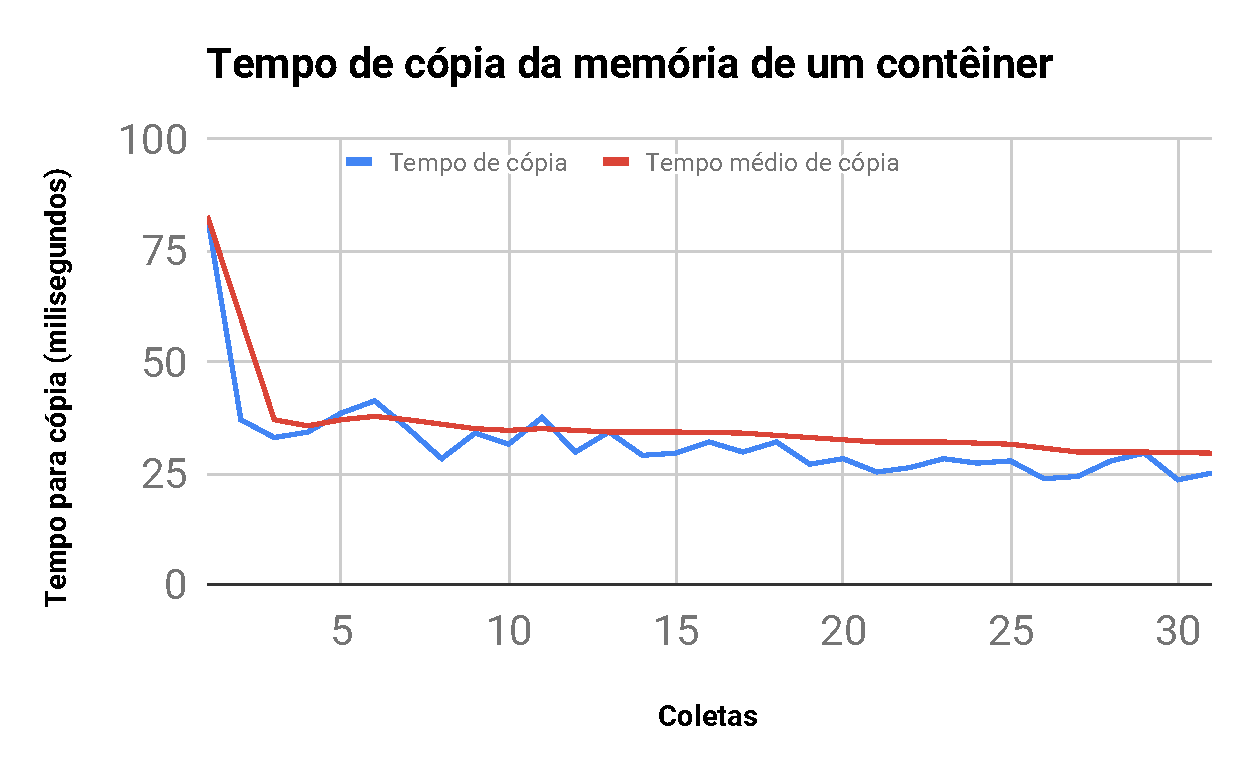
\includegraphics[scale=0.70]{memoria-copia.pdf}
\centering
\label{fig:memoria-copia}
\begin{center}
Fonte: Próprio autor 
\end{center}
\end{figure}


Outra preocupação é o tempo de transporte das evidências para o armazenamento fora da nuvem.
%
Caso o transporte da evidência leve mais tempo que a geração do próximo instantâneo, um \textit{backlog} de transporte se formará levando a perdas nas evidências que estejam pendentes para transporte.
%
Para avaliar esse impacto, durante o experimento foram medidos os tempos de transporte das evidências para o armazenamento fora da nuvem.
%
Os resultados são mostrados no gráfico da Figura \ref{fig:evidencia_transporte}.
%
É possível notar que o tempo de transporte estabiliza após atingido o tamanho da janela. O tempo de transporte da evidência fica, em média próximo dos 30 segundos. 

\begin{figure}[htb!]
\footnotesize
\caption{Tempo de transporte da evidência}
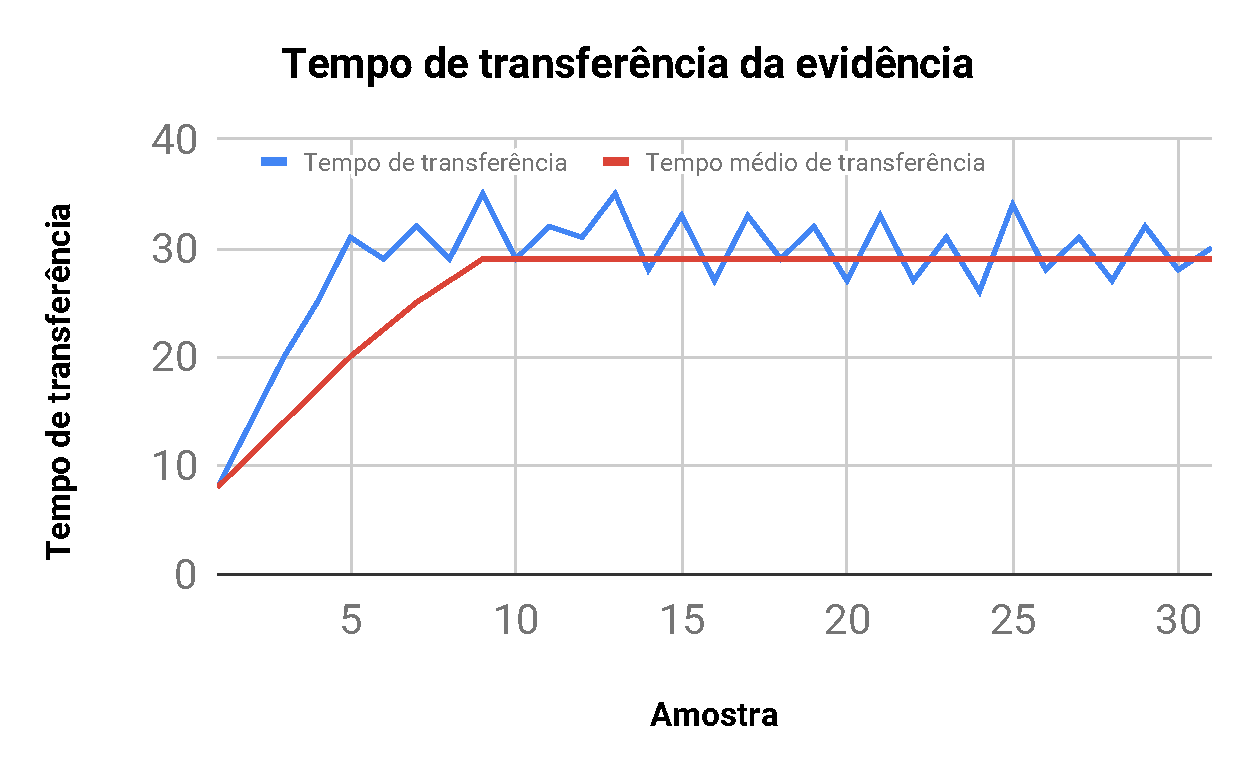
\includegraphics[scale=0.70]{evidencia-download.pdf}
\centering
\label{fig:evidencia_transporte}
\begin{center}
Fonte: Próprio autor 
\end{center}
\end{figure}


%
Tanto a topologia quando a arquitetura do transporte da evidência e a arquitetura do que se deseja extrair a evidência como a quantidade de contêiners, distribuição geográfica dos hospedeiros, tamanho da evidência de memória, entre outros, são fatores que contribuem tanto positiva quando negativamente no tempo de transporte.
%
Neste experimento o gerador de evidências, um motor de páginas dinâmicas composto por 3 contêiners, está na América do Norte enquanto que a máquina física para onde as evidências foram transportadas e que é responsável pelo transporte da evidência está na América do Sul.
%
Aplicações web modernas compostas por vários microserviços implementados em conteiners \cite{StubbsConteinersNumberMicroServices:2015}, podem elevar o tempo necessário para \fancyname coletar evidências suficientes de modo a ter uma visão do estado da aplicação em um momento $t$.

\subsection{Identificação de injeção de código malicioso}
\label{sec:proposta-exp-malware}

Um segundo experimento teve como objetivo determinar se é possível, através da análise das evidências coletadas, identificar injeção de código malicioso na memória do contêiner.
%
Para este fim uma biblioteca \textbf{libexample.so} simulando um código malicioso foi injetado em um dos contêineres.
%
Após cinco minutos de \fancyname realizando coletas, uma biblioteca foi injetada na memória de um dos contêineres. Após a injeção permitiu-se que a solução continuasse coletando por mais 5 minutos.
%
Além da coleta do conteúdo do diretório \textbf{/proc/pid/numa\_maps}, realizou-se também uma cópia crua da memória do processo do contêiner utilizando o utilitário \textit{nsenter} via comando descrito na Figura \ref{fig:comando-copia}.
%

%A primeira tentativa de cópia do conteúdo da memória de um contêiner usando o utilitário \textit{GDB} diretamente não foi bem sucedida. 
%
%Segundo \cite{cgroupsxptrace}, chamadas de systema usadas por ferramentas como \textit{GDB} foram criadas antes da implementação de \textit{cgroups} e \textit{namespaces} no núcleo do Linux e portanto não estão cientes do isolamento entre os processos de um contêiner e de seu hospedeiro.
%
%Quando \textit{GDB} usa a chamada de sistema \textit{ptrace} para acessar uma área de memória isolada por \textit{cgroups}, o núcleo gera um sinal de violação impledindo o acesso a memória.
%
%Por isso o utilitário \textit{nsenter} foi usado.

\begin{figure}[htb!]
\footnotesize
\caption{Comando para cópia crua da memória do processo do contêiner}
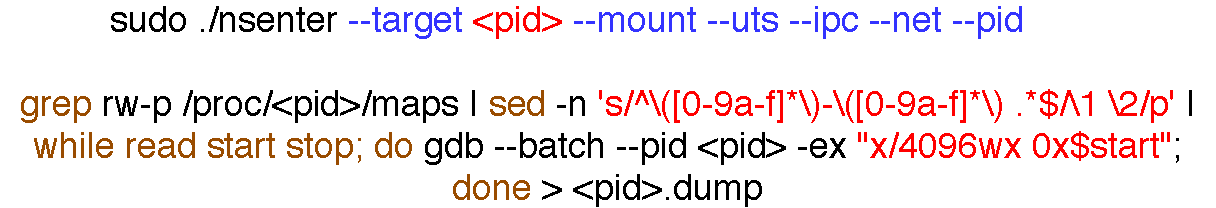
\includegraphics[scale=0.60]{comando-copia-memoria-gdb.pdf}
\centering
\label{fig:comando-copia}
\begin{center}
Fonte: Próprio autor 
\end{center}
\end{figure}

%
De posse das coletas do diretório \textbf{/proc/pid/numa\_maps} comparou-se dois momentos distintos na vida do contêiner, antes e depois da injeção da biblioteca.
%
Observando as Figuras \ref{fig:antes-injecao} e \ref{fig:apos-injecao} é possível notar que no instantâneo após a injeção aparece a biblioteca \textbf{libexample.so} simulando o código malicioso entre os endereços \textbf{7f85631b8000} e \textbf{7f85633b9000}.
%
Logo, é possível identificar a injeção de um código malicioso via evidência coletada por \fancyname do diretório \textbf{/proc/pid/numa\_maps}, permitindo-se por exemplo que ataques de injeção de código sejam identificados.
%
A Figura \ref{fig:conteudo-memoria-copia-gdb} mostra o conteúdo da parte legível da memória no endereço \textbf{0x7f85633b9000} onde a biblioteca \textbf{libexample.so} simulando um código malicioso está alocada.

\begin{figure}[htb!]
\footnotesize
\caption{Parte do arquivo \textbf{/proc/pid/numa\_maps} ANTES da injeção }
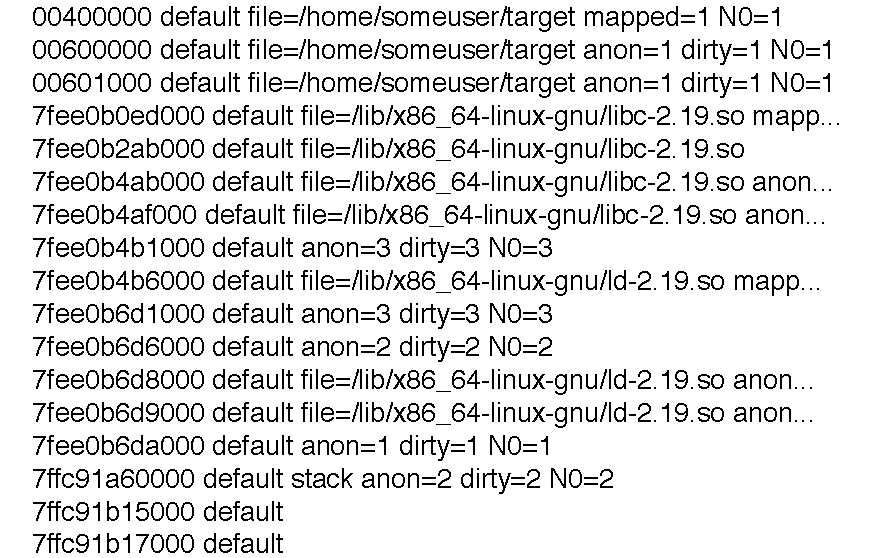
\includegraphics[scale=0.80]{antes-injecao.pdf}
\centering
\label{fig:antes-injecao}
\begin{center}
Fonte: Próprio autor 
\end{center}
\end{figure}


\begin{figure}[htb!]
\footnotesize
\caption{Parte do arquivo \textbf{/proc/pid/numa\_maps} APÓS a injeção }
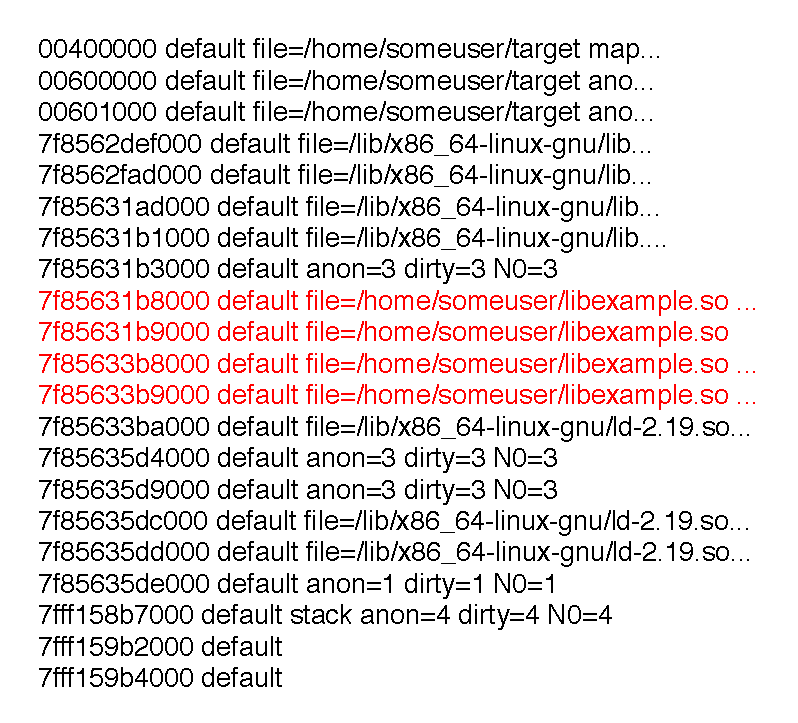
\includegraphics[scale=0.80]{apos-injecao.pdf}
\centering
\label{fig:apos-injecao}
\begin{center}
Fonte: Próprio autor 
\end{center}
\end{figure}

%
As primeiras tentativas de cópia do conteúdo da memória do processo do contêiner foram feitas via \textit{ptrace} e não obteve sucesso. 
%
Segundo \cite{cgroupsxptrace} isto ocorre pois as chamadas de sistema que ferramentas como \textit{ptrace} e \textit{htop} usam foram criadas antes da implementação de \textit{cgroups} no \textit{kernel} do linux e sendo assim não tem consciência da existência de isolamento entre processos.
%
Quando o \textit{ptrace} tenta acessar uma área de memória isolada por \textit{cgroups}, o \textit{kernel} envia um sinal de violação de acesso de memória.%, o resultado é mostrado na Figura \ref{fig:erro-copia-gdb}.
%

A documentação do Docker \cite{capabilities} menciona o comando \texttt{--cap-add=SYS_PTRACE --security-opt-seccomp=unconfined} que permite que o \textit{ptrace} consiga acessar a memória de um processo dentro do contêiner mas não permite que a máquina hospedeira ou outro contêiner tenha acesso (referência).
%
Ainda segundo \cite{cgroupsxptrace} uma alternativa para viabilizar a monitoração e acesso a informações de memória seria o de expor tais informações na estrutura de \textbf{/sys/fs/cgroup/} da mesma forma que é feita para \textbf{/proc/pid/}.
%
O sucesso na cópia do conteúdo da memória do processo do contêiner só foi alcançado quando utilizou-se a ferramenta \textit{nsenter}.
%

\begin{figure}[htb!]
\footnotesize
\caption{Conteúdo da memória de \textbf{libexample.so} no formato [endereço]: [conteúdo]}
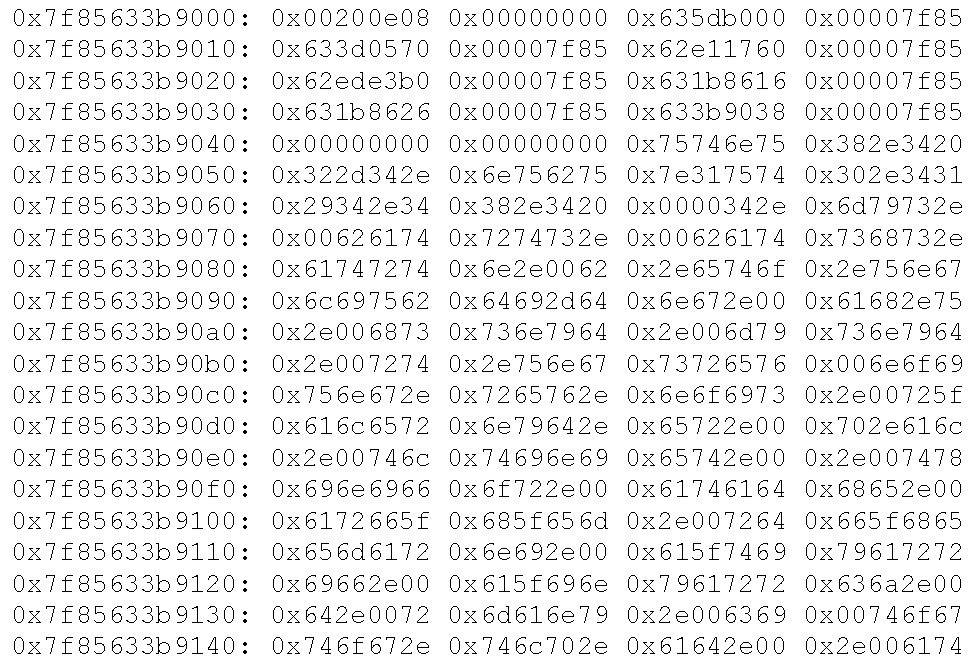
\includegraphics[scale=0.65]{conteudo-memoria-copia-gdb.pdf}
\centering
\label{fig:conteudo-memoria-copia-gdb}
\begin{center}
Fonte: Próprio autor 
\end{center}
\end{figure}


%\begin{figure}[htb!]
%\footnotesize
%\caption{Tentativa mal sucedida de cópia do conteúdo da memória}
%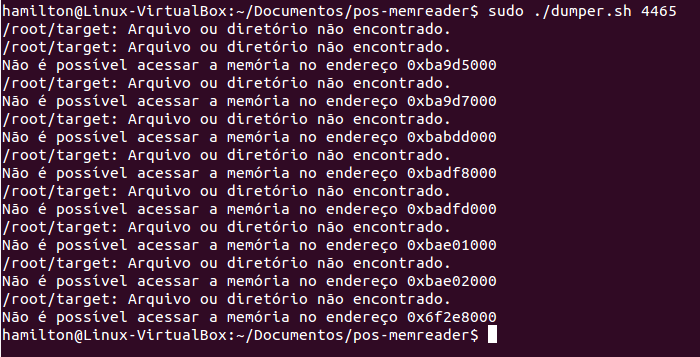
\includegraphics[scale=0.65]{nao-consido-dumpar-memoria.png}
%\centering
%\label{fig:erro-copia-gdb}
%\begin{center}
%Fonte: Próprio autor 
%\end{center}
%\end{figure}



\section{Limitações}
\label{sec:proposta-limit}

A proposta descrita pede que o recurso em nuvem seja identificável de forma única a fim de realizar a associação entre evidência e sua origem.
%
Durante o curso deste projeto essa identificação única só foi possível através do hash da imagem do contêiner. Este foi o único recurso que, submetido ao processo de construção a partir da mesma receita resultou no mesmo \textit{hash} da imagem.
%
Assim, a implementação para verificação da solução proposta consegue apenas coletar informações de memória no espaço do usuário (\textit{user space}), ela não consegue acessar o espaço de núcleo do sistema operacional (\textit{kernel space}). 
%
A implementação de \fancyname neste documento em princípio não consegue investigar códigos malicioso que se baseiam em informações do \textit{kernel space}.
%
Isso inclui, por exemplo, a comparação de informações do PEB (\textit{Process Environment Block} -- Bloco para o Ambiente dos Processos), que ficam no \textit{user space}, com informações do VAD (\textit{Virtual Address Descriptor} -- Descritor de Endereços de Memória Virtual), que fica no \textit{kernel space}. 
%
%Análise de ameaças do tipo DKOM ( \textit{Direct Kernel Object Manipulation} -- Manipulação Direta dos Objetos do Kernel ) também não se beneficiam com a solução aqui proposta. 
%\marcosT{Não entendi a ``associação com o contêiner'' aqui. Você quer dizer que ``não se beneficiam com a solução aqui proposta'' ou outra coisa? Você não definiu o que seria a tal ``associação com o contêiner'' fora do contexto da sua solução, então ficou confuso - Hamilton: Feito}.

Como mencionado em \cite{CaseMemoryForensics:2014}, ``para uma análise eficiente de um incidente em memória, são necessárias cópias da mesma \textbf{antes e depois} do incidente.''
%
Outra limitação da solução proposta é a necessidade da mesma estar instalada no sistema sob investigação a priori para que os resultados descritos neste documento sejam alcançados.
%
Como há uma ampla variedade de ameaças digitais ao largo e novas são criadas constantemente, caso o sistema de detecção de ameaça ao qual \fancyname está integrado não conseguir detectar um ataque em andamento, evidências importantes para descrever o sistema antes do ataque podem ser perdidas no descarte do limite da janela.


\chapter{Conclusões e recomendações para trabalhos futuros}
\label{sec:proposta-concl-recom}

%
Neste capítulo são apresentadas as conclusões do presente trabalho e as recomendações para a continuidade dos trabalhos neste campo de estudo.

\section{Conclusões}
\label{sec:proposta-concl}

%\marcosT{Uma boa conclusão retoma, logo na primeira frase, o problema que ela se propunha a resolver. Comece com uma ou mais frases nesse sentido, (nota: \textbf{sem} copiar+colar de outro ponto do texto). - Hamilton: Feito} \marcosT{Só que não: eu disse para você retomar o \textbf{problema} na sua primeira frase. Sua frase começa retomando a \textbf{solução}. Essa que você colocou como primeira seria boa como uma segunda frase, em que você reforça como resolve o problema - Hamilton: Acho que agora foi :)}
%
Ameaças digitais que atuam diretamente na memória de sistema não costumam deixar rastros em disco após terem os recursos correspondentes desalocados, dificultando análises forenses posteriores.
%
Esse problema é especialmente notável em sistemas de computação em nuvem, nos quais a alocação e desalocação de recursos virtualizados (e.g., VMs e contêineres) é frequente.
%
Essa característica, aliada a aspectos como multi-inquilinato e multi-jurisdição de nuvens computacionais, dificulta a coleta de evidências para a investigação de incidentes.

%
Nesse cenário, a proposta apresentada visa relacionar o instantâneo de memória a sua origem, utilizando o \textit{hash} calculado do recurso computacional em nuvem como identificador da origem da evidência armazenada.
%
Para evitar uso excessivo de memória, a quantidade de dados armazenados usa uma janela de armazenamento, o que permite descrever a memória antes e depois de um ataque (e.g., de injeção de memória). 
%
Transportando de forma segura e armazenando a evidência em local conhecido fora da nuvem, evitam-se os problemas relacionados a multi-jurisdição e multi-inquilinato das nuvens computacionais.
%
A comparação de instantâneos de memória coletados em diferentes instantes de tempo permite a identificação de injeção de código assim como extrair o conteúdo da parte legível do endereço de memória correspondente.

%
Combinada com uma ferramenta para identificação de ameaças, essas características de \fancyname o transformam em uma solução poderosa para prover evidências e, assim, viabilizar análises forenses na nuvem.

\section{Trabalhos Futuros}
\label{sec: proposta-trab-fut}

%
Como mencionado em \ref{sec:proposta-limit} a solução proposta é capaz de gerar evidências de memória apenas do espaço do usuário (\textit{user space}). 
%
Alguns códigos malicioso injetados em memória são capazes de manipular o retorno de funções do kernel. Recomenda-se para trabalhos futuros a incorporação à \fancyname uma forma de realizar a extração do conteúdo de memória do espaço do kernel (\textit{kernel space}).


\bibliographystyle{abntex2-alf}
\bibliography{bibliography}

\appendix

%\input{appendices/conversion.tex}

\end{document}
